% Generated by paper/build/build_arxiv.py from the pinned
% paper/latex_export/main.tex. Do not edit this file directly.
% Pinned source SHA-256: 3679E5178CBDC041B1FF63E7CE9F930A613DCE255D3BB762B769DB1F06CAB468
% arXiv layout: 1-inch margins, letter paper, 10 pt.

% Options for packages loaded elsewhere
\PassOptionsToPackage{unicode}{hyperref}
\PassOptionsToPackage{hyphens}{url}
\documentclass[
  10pt,
]{article}
\usepackage{xcolor}
\usepackage[margin=1in,letterpaper]{geometry}
\usepackage{amsmath,amssymb}
\setcounter{secnumdepth}{-\maxdimen} % remove section numbering
\usepackage{iftex}
\ifPDFTeX
  \usepackage[T1]{fontenc}
  \usepackage[utf8]{inputenc}
  \usepackage{textcomp} % provide euro and other symbols
\else % if luatex or xetex
  \usepackage{unicode-math} % this also loads fontspec
  \defaultfontfeatures{Scale=MatchLowercase}
  \defaultfontfeatures[\rmfamily]{Ligatures=TeX,Scale=1}
\fi
\usepackage{lmodern}
\ifPDFTeX\else
  % xetex/luatex font selection
\fi
% Use upquote if available, for straight quotes in verbatim environments
\IfFileExists{upquote.sty}{\usepackage{upquote}}{}
\IfFileExists{microtype.sty}{% use microtype if available
  \usepackage[]{microtype}
  \UseMicrotypeSet[protrusion]{basicmath} % disable protrusion for tt fonts
}{}
\makeatletter
\@ifundefined{KOMAClassName}{% if non-KOMA class
  \IfFileExists{parskip.sty}{%
    \usepackage{parskip}
  }{% else
    \setlength{\parindent}{0pt}
    \setlength{\parskip}{6pt plus 2pt minus 1pt}}
}{% if KOMA class
  \KOMAoptions{parskip=half}}
\makeatother
\usepackage{longtable,booktabs,array}
\usepackage{caption}
\newcounter{none} % for unnumbered tables
\usepackage{calc} % for calculating minipage widths
% Correct order of tables after \paragraph or \subparagraph
\usepackage{etoolbox}
\makeatletter
\patchcmd\longtable{\par}{\if@noskipsec\mbox{}\fi\par}{}{}
\makeatother
\usepackage{graphicx}
\makeatletter
\newsavebox\pandoc@box
\newcommand*\pandocbounded[1]{% scales image to fit in text height/width
  \sbox\pandoc@box{#1}%
  \Gscale@div\@tempa{\textheight}{\dimexpr\ht\pandoc@box+\dp\pandoc@box\relax}%
  \Gscale@div\@tempb{\linewidth}{\wd\pandoc@box}%
  \ifdim\@tempb\p@<\@tempa\p@\let\@tempa\@tempb\fi% select the smaller of both
  \ifdim\@tempa\p@<\p@\scalebox{\@tempa}{\usebox\pandoc@box}%
  \else\usebox{\pandoc@box}%
  \fi%
}
% Set default figure placement to htbp
\def\fps@figure{htbp}
\makeatother
\setlength{\emergencystretch}{3em} % prevent overfull lines
\providecommand{\tightlist}{%
  \setlength{\itemsep}{0pt}\setlength{\parskip}{0pt}}
% header.tex -- build-only preamble for the seam manuscript draft.
% Not part of the manuscript; passed with --include-in-header.
% Assumes the Pandoc XeLaTeX template has already loaded fontspec,
% unicode-math, longtable, booktabs, array, caption, calc, etoolbox.

% ---------------------------------------------------------------------
% 1. Unicode text-mode glyphs that Latin Modern Roman does not carry.
%    Each is mapped to the equivalent math macro, so it typesets from
%    Latin Modern Math and stays searchable/copyable in the PDF only
%    where the source glyph survives (math macros are not ToUnicode).
%    U+2605 (★) has no Latin Modern Math glyph, so it maps to the
%    Latin Modern Math star operator U+22C6 (\star) rather than pulling
%    in a platform symbol font. No Segoe UI Symbol fallback remains.
% ---------------------------------------------------------------------
\usepackage{newunicodechar}
% unicode-math installs its own begin-document definitions for math
% characters, so the mappings must be declared inside \AtBeginDocument
% to run after them; a plain preamble \newunicodechar is overwritten.
\AtBeginDocument{%
  \newunicodechar{★}{\ensuremath{\star}}%
  \newunicodechar{⊆}{\ensuremath{\subseteq}}%
  \newunicodechar{→}{\ensuremath{\rightarrow}}%
  \newunicodechar{ρ}{\ensuremath{\rho}}%
  \newunicodechar{π}{\ensuremath{\pi}}%
  \newunicodechar{∩}{\ensuremath{\cap}}%
  \newunicodechar{τ}{\ensuremath{\tau}}%
  \newunicodechar{≔}{\ensuremath{\mathrel{:=}}}%
  \newunicodechar{⊓}{\ensuremath{\sqcap}}%
  \newunicodechar{∧}{\ensuremath{\wedge}}%
  \newunicodechar{∈}{\ensuremath{\in}}%
  \newunicodechar{≡}{\ensuremath{\equiv}}%
  \newunicodechar{′}{\ensuremath{{}^{\prime}}}%
}

% ---------------------------------------------------------------------
% 2. Captions. The manuscript writes its own "**Figure 1.**" label in
%    the caption text, so suppress LaTeX's "Figure 1:" prefix to avoid
%    a duplicated label. Table captions are ordinary body paragraphs
%    (Pandoc pipe tables carry no \caption), so this only affects figures.
% ---------------------------------------------------------------------
\captionsetup{labelformat=empty,justification=raggedright,singlelinecheck=false,font=small}

% ---------------------------------------------------------------------
% 3. Tables. Sixteen pipe tables become sixteen longtables. Long arm
%    names in \texttt cannot hyphenate, so widen the usable measure by
%    shrinking table type and inter-column padding.
% ---------------------------------------------------------------------
\AtBeginEnvironment{longtable}{\footnotesize}
\setlength{\tabcolsep}{3pt}
\renewcommand{\arraystretch}{1.12}
\setlength{\LTpre}{6pt}
\setlength{\LTpost}{6pt}

% ---------------------------------------------------------------------
% 4. Floats: keep figures near their references in a single-column draft.
% ---------------------------------------------------------------------
\usepackage{float}
\floatplacement{figure}{htbp}
\renewcommand{\topfraction}{0.92}
\renewcommand{\bottomfraction}{0.8}
\renewcommand{\textfraction}{0.08}
\renewcommand{\floatpagefraction}{0.75}

% Keep mechanism names whole; the Section 2 heading otherwise breaks
% SentinelAgent as "Sen-tinelAgent".
\hyphenation{sentinelagent}
\hyphenation{tracegrant}

% ---------------------------------------------------------------------
% 5. Author block. Pandoc escapes backslashes in YAML author metadata,
%    so set the multi-line display form after the template has run.
% ---------------------------------------------------------------------
\AtBeginDocument{%
  \author{Prathamesh N Patil\\Department of Computer Engineering\\Sardar Patel Institute of Technology}%
  \hypersetup{pdfauthor={Prathamesh N Patil}}%
}

% --- variant B: long code spans are wrapped selectively by the build
%     post-process, not globally; global seqsplit breaks status tokens
%     such as SUPPORTED mid-word.
\usepackage{seqsplit}
\usepackage{url}
\usepackage{needspace}
\let\origtexttt\texttt
% Inline code and artifact paths stay upright even inside italic notes.
% \upshape changes only the shape, so bold table/heading contexts keep their
% weight.  The url package's \path command selects \UrlFont directly, so it
% needs the same rule.
\renewcommand{\texttt}[1]{{\upshape\origtexttt{#1}}}
\makeatletter
\def\url@ttstyle{\def\UrlFont{\ttfamily\upshape}}
\makeatother
\setlength{\emergencystretch}{4em}
% Overfull boxes are counted from the log; do not print debug rules in the
% candidate PDF (they read as black artifacts in narrow table columns).
\overfullrule=0pt

% --- variant C: allow a break before escaped underscores in plain text
%     so lines do not end with a trailing underscore.
\let\origunderscore\_
\renewcommand{\_}{\allowbreak\origunderscore}

% --- variant F: inside longtables, use the original \texttt so cells
%     break only at separators, not mid-token.
\AtBeginEnvironment{longtable}{\let\texttt\origtexttt}

\usepackage{bookmark}
\IfFileExists{xurl.sty}{\usepackage{xurl}}{} % add URL line breaks if available
\urlstyle{same}
% fallback for those not using the hyperref driver hyperxmp:
\makeatletter
\@ifundefined{xmpquote}{\newcommand{\xmpquote}[1]{#1}}{}
\makeatother
\hypersetup{
  pdftitle={The Handoff Nobody Owns: Measuring What Cross-Mechanism Authorization Seams Cannot Carry},
  pdfauthor={Prathamesh N Patil},
  pdfkeywords={\xmpquote{cross-mechanism authorization; agent
authorization; authorization seams; scope narrowing; evidence carriage;
conformance testing; locked-artifact methodology}},
  hidelinks,
  pdfcreator={LaTeX via pandoc}}

\title{The Handoff Nobody Owns: Measuring What Cross-Mechanism
Authorization Seams Cannot Carry}
\author{Prathamesh N Patil}
\date{8 November 2026}

\begin{document}
\maketitle

\begin{abstract}

Agent authorization rarely stops at a mechanism boundary: a sender
narrows authority, a bridge translates it into a record the receiver can
read, and the receiver applies admission rules. Each can be correct
alone while the composition admits a call the sender never authorized.
This paper treats that handoff as a measurement problem, separating two
questions: whether the composed system commits a sender-relative
violation, and whether composition adds a failure the receiver-only arm
does not exhibit. Predictions, cases, arms, and hashes are recorded in
internal locks before execution; values are script-checked against
stored artifacts. Across 2,446 executions, the composed arms admit 24/40
and 28/48 sender-unauthorized calls in the two pair pilots, but the
receiver-only arms admit the same calls; receiver-relative novelty is
zero in both, and both zeroes are forced by our translation layers: the
TraceGrant-side contract is built per call from the requested tool, and
the SentinelAgent-side token is minted directly into a fresh registry.
An action-narrowing family illustrates the limit: the receiver contracts
are byte-identical in the receiver-only and composed arms, and a 4/4
receiver-relative count appears only under a scoring rule recorded after
the data. Non-narrowing-preserving derivations leak four new cases per
variant, standalone and composed, locating the fault at the bridge. We
close with a replication package and a repair taxonomy: consumption or
evidence carriage when the narrowed fact reaches the decision,
derivation repair when the bridge widens. The zero is a recorded
property of narrowing-preserving mappings on the frozen cases, not a
theorem.

\textbf{Keywords:} cross-mechanism authorization; agent authorization;
authorization seams; scope narrowing; evidence carriage; conformance
testing; locked-artifact methodology

\end{abstract}

\section{1. Introduction}\label{introduction}

A sender holds authority over a call space and narrows it before handing
a call to another mechanism. A bridge translates the narrowed decision
and the current state into a record the receiver can read. The receiver
applies its own admission rules. Each party can be faithful inside its
own world --- the narrowing exact, the transport byte-perfect, the
receiver's verdict consistent with its own policy --- and the composed
system can still admit a call the sender never authorized. The failure
is not necessarily an unfaithful record. It can be a faithful record
that carries a fact the receiver's decision never reads.

A concrete instance motivates the paper. In the E1 action-narrowing
family (Section 4.2), the sender's root authority includes
\texttt{send\_external}, the narrowed authority does not, and the bridge
builds a receiver-side contract from the requested tool rather than from
the narrowed action set. The narrowed action set is present in the
composed snapshot, but it is not represented in the contract the
receiver decides on: the contract is byte-identical in the receiver-only
and composed arms. The composed arm admits \texttt{send\_external} on
all four attack cases because the bridge never presents the narrowed
action set to the receiver's decision. This is a bridge-construction
failure, not a receiver that reads a carried fact incorrectly. We call
the handoff the seam: the boundary between a sender's narrowing and a
receiver's decision, owned by neither mechanism.

The research question is sender-relative: at a cross-mechanism handoff,
does the composed system enforce the sender's narrowing, or does it
admit calls the narrowing never conferred? The measurement question is
narrower: does composition add an admission beyond what the standalone
receiver already exhibits? The two questions coincide only when the
receiver is safe on its own. When the receiver already admits the call,
the composed system commits a sender-relative violation but adds no
receiver-relative novelty. This paper reports both counts separately;
the distinction is the main methodological correction of the study.

\textbf{Contributions.} The paper makes four contributions.

\begin{enumerate}
\def\labelenumi{\arabic{enumi}.}
\tightlist
\item
  \textbf{A locked-artifact method for cross-mechanism seams.} Primary
  predictions, cases, arms, and input hashes are recorded in internal
  locks before execution; later scoring norms and prediction overrides
  are dated and disclosed (Sections 3.1, 4.2, 4.3, 7.2); runs are
  sequential, offline, and deterministic; predicted-versus-observed
  discrepancies are reconciled verbatim; and every reported number is
  transcribed and script-checked against stored artifacts (Section 3.1).
\item
  \textbf{A two-reading seam test.} The test separates a sender-relative
  violation (the sender denies, the composed system admits) from
  receiver-relative novelty (the standalone receiver denies, the
  composed system admits). It also records what the receiver's decision
  reads, not merely what the record carries (Sections 3.2--3.3).
\item
  \textbf{An empirical map of four frozen experiment sets.} Across 2,446
  executions, the two pair pilots show that the composed arms admit
  24/40 and 28/48 sender-unauthorized calls, while the receiver-only
  arms admit the same calls; receiver-relative novelty is zero, and
  those two zeroes are forced by the author-built bridges. The
  translation layers are ours: the TraceGrant-side contract is built per
  call from the requested tool, and the SentinelAgent-side token is
  minted directly into a fresh registry. The E1 action family is an
  illustration of the limit, not a composition-specific result: the
  receiver contracts are byte-identical in the receiver-only and
  composed arms, and the 4/4 count appears only under a scoring rule
  recorded after the E1 records existed. The boundary study shows that
  non-narrowing-preserving bridge derivations leak four new cases per
  variant both standalone and composed (Sections 4.1--4.5).
\item
  \textbf{A repair taxonomy and a replication package.} The taxonomy
  separates three receiver-side repairs (evidence carriage; retention of
  the upstream denial; action-scope consumption) from the bridge-side
  derivation rule. Action-scope consumption can be implemented as a
  pre-synthesis check over the snapshot or as a restriction of the
  synthesized contract's MAY set, which the lock records as
  decision-equivalent; Test 2 measured the pre-synthesis form. The
  package contains the frozen case sets, harnesses, locks, and protocol;
  it is a release candidate, not a public conformance service (Sections
  5 and 8).
\end{enumerate}

\textbf{What the paper does not claim.} The zero is a recorded property
of narrowing-preserving mappings on the frozen case sets, not a theorem,
and it is not a claim that seams are safe in general. The paper does not
claim that APC, TraceGrant, or SentinelAgent is broken; their published
guarantees are reported as their authors state them. It does not claim
benchmark comparability, production safety for any repair arm, or
authenticated transport for the HMAC test channel. Two hypotheses, H4
(shared audit trail) and H7 (intent layer), remain \texttt{UNTESTED}
(Section 7.5). The broader attenuation and delegation literature is
outside the measurement scope; the contribution is a cross-mechanism
measurement, not a new attenuation primitive (Section 6).

\textbf{Roadmap.} Section 2 places the three formal spines and Progent.
Section 3 presents the method, formal core, two-reading seam test,
scoring conventions, execution ledger, threat model, and hypothesis key.
Section 4 reports the four experiment sets. Section 5 draws the repair
taxonomy and the practical implications. Section 6 positions the work,
Section 7 states the threats and open hypotheses, Section 8 describes
the replication package, and Section 9 concludes.

The formal objects are simple. A call space C collects calls c = (tool,
resource, arguments, \ldots). A mechanism M = (V\_M, admit\_M) comprises
a vocabulary V\_M --- the fields the mechanism can represent and,
structurally, read --- and an admission function admit\_M(c, ρ) ∈
\{allow, deny\}. Authority A ⊆ C is the call set a principal confers; a
sender narrows A to A′ ⊆ A. A bridge B consumes the narrowed decision
and state and writes the receiver-side record \mbox{ρ\_R} = B(A′, state).
Composition is admit\_C(c) ≔ admit\_R(c, B(A′)), and the composition's
effective authority is A\_C ≔ \{ c : admit\_C(c) = allow \}. The
receiver's read set V\_read ⊆ V\_R is the set of fields its decision
actually consults --- not the fields the record carries, but the fields
the decision reads.

\begin{figure}
\centering
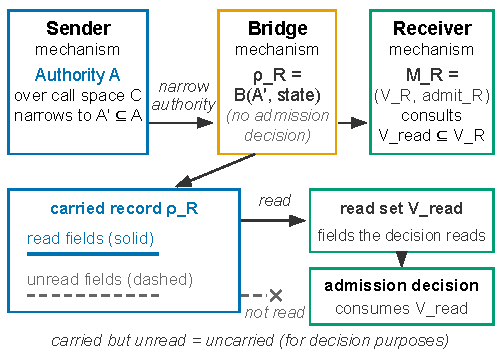
\includegraphics[width=3.33in,height=\textheight,keepaspectratio,alt={Figure
1. Anatomy of a cross-mechanism handoff --- the sender narrows
authority, the bridge translates it into a receiver-side record, and the
receiver decides; the schematic distinguishes the record the bridge
carries from the read set the receiver's decision actually
consults.}]{figures/figure_1_handoff_anatomy.pdf}
\caption{\textbf{Figure 1.} Anatomy of a cross-mechanism handoff --- the
sender narrows authority, the bridge translates it into a receiver-side
record, and the receiver decides; the schematic distinguishes the record
the bridge carries from the read set the receiver's decision actually
consults.}\label{fig:figure1}
\end{figure}

The schematic carries no data and no numbers. A fact in the carried
record that no decision reads constrains no decision; Section 3.2 states
this as a definitional observation, not an empirical result. The seam
can therefore admit what the sender never narrowed even when the
transport is clean.

\section{2. Background --- APC (Agentic Principal Chain), TraceGrant,
SentinelAgent; Progent as
reference}\label{background-apc-agentic-principal-chain-tracegrant-sentinelagent-progent-as-reference}

This section places the three formal spines whose within-mechanism
guarantees leave the cross-mechanism slot uncovered, and it reports each
upstream guarantee as its authors' self-report --- never upgraded to a
manuscript result and never cited as this program's measurement. None of
the three spines supplies a cross-mechanism composition guarantee; the
observation is scoped to these three systems and is not a universal
negative. The purpose is to show where each guarantee stops, so that the
uncovered slot --- the seam between mechanisms --- can be named plainly.

APC {[}APC{]} --- the Agentic Principal Chain mechanism --- reports
within-mechanism authorization: a scope algebra with meet ⊓, conditions
C1--C6, and Thm 4.7 (Composition Soundness), conditional on a complete
effective restriction set, serialized admission, and a static X within a
session. APC's ``composition'' is composition of action sequences inside
one session; it is not composition across mechanisms. Its resource meet
holds inside the mechanism. APC alone governs calls inside one
mechanism; it says nothing about what happens when a narrowed call
crosses into another mechanism's vocabulary, and it supplies no
cross-mechanism composition guarantee. Its authorization reasoning is
sound only relative to the assumptions the theorem names, and nothing in
APC extends that reasoning across a bridge to a receiver with a
different vocabulary.

TraceGrant {[}TraceGrant{]} reports contract-governed task-effect
authorization: POEC contracts, Eq. 2 / Algorithm 1. Its Eq. 10 is a
contract-soundness assumption, assessed empirically in its §5.4, not
proven. Like APC, TraceGrant's guarantee stays inside its own mechanism
and extends no composition claim across a seam. Contract soundness is an
assumption of the formalism, not a result this program verifies, and it
covers calls handled within TraceGrant's own contract model rather than
calls handed off to another mechanism.

SentinelAgent {[}SentinelAgent{]} reports a token model τ with
principles P1--P7 (P1 and P3--P7 TLA+-checked; P2 probabilistic), a TLA+
model of 2.7M states --- an upstream self-report, not a measurement of
this program --- and Thm 4 (Composition Safety with Write-Impact
Notification), which is stated for two delegation chains that both
satisfy P1--P7 within its own framework. It does not state a guarantee
for a chain handed to a different mechanism's decision procedure; that
boundary is where this paper's cross-mechanism question begins. That
figure is the authors' own model-scale claim; this program neither
measured it nor relies on it as evidence.

The uncovered slot: within-mechanism guarantees do not compose across
mechanisms. None of APC, TraceGrant, or SentinelAgent supplies a
cross-mechanism composition guarantee. Scoped to these three --- no
universal negative --- the slot remains: what happens at the seam
between a sender's narrowing and a receiver's decision when the two
mechanisms do not share a vocabulary or a decision rule.

The three scopes differ in their limits, but they share the same
boundary. APC's theorem is conditional on a static X and governs
intra-session action-sequence composition inside one mechanism, so it
says nothing about a call crossing into another mechanism's vocabulary.
TraceGrant's soundness is assumed, not proven (Eq. 10), so its
delegation guarantee covers contracts handled within TraceGrant's own
model, not calls handed off to another mechanism. SentinelAgent's
theorem addresses composition of two chains within its own P1--P7
framework, not a chain handed to a different mechanism's decision
procedure, so the cross-mechanism case falls outside it.

Each guarantee stops at its mechanism's edge. A record can be faithful
at the bridge and still carry nothing the receiver's decision reads. A
signature can be valid and still attest nothing about the source of
authority. A theorem conditioned on a static state says nothing about a
dynamic handoff.

This paper's position is adjacent to that slot: narrowing-preservation
plus the blindness observation --- cross-mechanism composition --- is
the measurement target. The observation says a fact carried but never
read constrains no decision; narrowing-preservation requires the
composed system to enforce at least the sender's narrowing on the
relevant family. Together they name the question the three spines leave
to the seam, and this program measures whether it holds on the frozen
case sets. The claim is deliberately scoped: it concerns these three
spines, these mappings, and these case sets, and it is not a universal
statement about every bridge or every mechanism pair.

Progent {[}Progent{]} is a close reference point rather than an input to
this program: it enforces monotonic confinement inside a single
privilege-control layer, where an SMT solver classifies each policy
update as a narrowing or an expansion; this paper asks whether a
comparable narrowing survives translation across a mechanism boundary.
Its reported results remain its authors' self-report and are not used as
an input or comparison here. Nothing about Progent is claimed or
measured in this section, and its results play no role in the paper's
measured claims.

Disclosures: say ``reports,'' never upgrade a self-report to an
established result; upstream guarantees and numbers stay self-reported;
nothing in this section impugns any upstream mechanism; no
production-safety claim; no benchmark comparability; citations are
pointers, not verified inputs. Citation keys are bracketed, and no
bibliographic detail is invented. The industry/standards citation layer
belongs to Section 6 and is not invoked here.

\textbf{Scope of positioning.} This is a measurement paper, not a survey
of authorization theory. Section 6 positions the work against the three
formal spines, the standards and systems that define the relevant
vocabulary (OAuth token exchange and rich authorization requests,
macaroons, object-capability systems, relationship-based access control,
proof-carrying authentication, and SPKI), the closest 2026
agent-delegation work, and the two nearest empirical relatives. Those
literatures contain the established vocabulary for attenuation, caveat
discharge, ambient authority, and policy intersection; this paper uses
that vocabulary but does not claim to extend it. The contribution is a
cross-mechanism measurement of three specific mechanisms and their
handoffs, plus a method and a replication package. A comparative
treatment would require running the comparison systems under a common
lock; none is run here.

Table 1 summarizes each formal spine and the scope of its composition
claim.

\textbf{Table 1.} Formal spine and composition-claim scope.

{\def\LTcaptype{none} % do not increment counter
\begin{longtable}[]{@{}
  >{\raggedright\arraybackslash}p{(\linewidth - 4\tabcolsep) * \real{0.3333}}
  >{\raggedright\arraybackslash}p{(\linewidth - 4\tabcolsep) * \real{0.3333}}
  >{\raggedright\arraybackslash}p{(\linewidth - 4\tabcolsep) * \real{0.3333}}@{}}
\toprule\noalign{}
\begin{minipage}[b]{\linewidth}\raggedright
System
\end{minipage} & \begin{minipage}[b]{\linewidth}\raggedright
Formal spine
\end{minipage} & \begin{minipage}[b]{\linewidth}\raggedright
Composition-claim scope
\end{minipage} \\
\midrule\noalign{}
\endhead
\bottomrule\noalign{}
\endlastfoot
APC & scope algebra, meet ⊓, conditions C1--C6, Thm 4.7 (Composition
Soundness) & within APC, intra-session; conditional on complete
restriction set, serialized admission, static X \\
TraceGrant & POEC contracts, Eq. 2 / Algorithm 1 & soundness assumed
(Eq. 10), not proven \\
SentinelAgent & token τ, P1--P7, TLA+ (2.7M states), Thm 4 (Composition
Safety) & within its own delegation framework; no cross-mechanism
handoff guarantee \\
\textbf{This paper} & narrowing-preservation + blindness observation &
cross-mechanism composition --- the question the others leave to the
seam \\
\end{longtable}
}

Table note: the SentinelAgent ``2.7M states'' cell is an upstream
self-report, not a measurement of this program; the TLA+ model covers P1
and P3--P7, while P2 (intent) is probabilistic.

\section{3. Method}\label{method}

This section presents the method as a contribution in its own right: a
measurement discipline for cross-mechanism authorization seams, built so
that the numbers it produces can be re-derived from locked artifacts by
an independent reader. Cross-mechanism authorization invites measurement
failures that are hard to detect after the fact: scoring conventions
chosen once the data are visible, and counts typed by hand into reports.
The method is designed against both. It combines an internally
time-stamped lock-before-run protocol with a run stage that executes
only against locked inputs; it generates every reported number from run
artifacts rather than typing it; it reconciles predicted and observed
outcomes verbatim rather than editing them into agreement; and it
submits the consolidated record to a model-assisted adversarial review
and a second quality-assurance pass before anything is frozen. The
section proceeds from that discipline (Section 3.1) through the formal
objects it measures (Section 3.2) and the seam-test predicate (Section
3.3) to the scoring conventions that govern every classification
(Section 3.4), the execution program and its ledger (Section 3.5), and
the scope the method accepts (Section 3.8). Outcomes are reported
nowhere in this section; where a sentence might otherwise forecast what
a run found, it is phrased as what the method does or as how a quantity
is defined.

\subsection{3.1 Lock-before-run by internal
timestamp}\label{lock-before-run-by-internal-timestamp}

Every experiment's case set, arm roster, harness, and primary
predictions are frozen and hashed before it runs; the lock record exists
before any execution begins, and the executed cases are the locked ones.
Where a scoring norm was recorded after a run, the record is dated and
the dependence is disclosed (Section 4.2). Lock records and their
fingerprints --- for datasets, case sets, and harnesses --- are part of
each run's artifact tree: for the E1 extension's dataset lock and the
discriminating tests' lock, for the SentinelAgent pair's lock and case
set, and for the boundary run's lock and harness. Execution is strictly
sequential, offline, and deterministic. Determinism is audited rather
than presumed: the protocol replays locked executions and compares them
against the originals, and in the SentinelAgent run the replay covered
20 executions with 0 mismatches.

A run then passes through the stages that discipline what may be said
about it:

\begin{verbatim}
lock freeze cases, arms, primary predictions, hashes — before any run
run strictly sequential, offline, deterministic
audit anchors: oracle reproduction, case-dict equality, field checks
reconcile predicted-versus-observed recorded verbatim; never edited in
publish all numbers transcribed and script-checked; byte-verbatim embeds
\end{verbatim}

The audit stage anchors a run's results to checks that an independent
reader can reconstruct: reproduction of the scoring oracle, equality of
the run's case dictionary against the locked cases, and field-level
validation of the run records. The reconciliation stage is the integrity
core of the method: whenever an observed outcome differs from a locked
prediction, the difference is recorded verbatim, whether or not it
favors the hypothesis under test, and it is not edited into agreement
afterwards. The publish stage closes the loop: every reported number is
transcribed from the stored artifacts and checked by script against
them, and where the prose embeds an artifact value, it embeds that value
byte-verbatim. A consequence adopted throughout: a total is written only
as the explicit sum of its enumerated components, and no rounded
aggregate is used in its place.

\subsection{3.2 The formal core}\label{the-formal-core}

The definitions in this subsection are measurement instruments: they
state what the program scores, not what any run observed. A call space C
collects calls c = (tool, resource, arguments, principal, session,
\ldots). A mechanism M = (V\_M, admit\_M) comprises a vocabulary V\_M
--- the fields the mechanism can represent and, structurally, read ---
and an admission function admit\_M(c, ρ) ∈ \{allow, deny\}, evaluated
over a call and a receiver-side record ρ. Authority A ⊆ C is the call
set a principal confers; a sender narrows A to A′ ⊆ A. A bridge B is the
seam's translation step: it consumes the narrowed decision together with
state and writes the receiver-side record \mbox{ρ\_R} = B(A′, state).
Composition is admit\_C(c) ≔ admit\_R(c, B(A′)), and the composition's
effective authority is A\_C ≔ \{ c : admit\_C(c) = allow \}.

The read set V\_read(ρ) ⊆ V\_M is the set of fields on which admit\_M
actually depends --- the support of the decision function, not the
fields the record carries. This distinction is the formal core's one
substantive definition. It yields a definitional observation:

\textbf{Blindness observation (definitional).} Fix a record ρ and a
family F. If admit\_R depends on c only through the projection
π\_\{V\_read\}(c, ρ), and no value in V\_read separates A′ ∩ F from its
complement on a pair of calls, then no admission function over V\_read
can enforce A′ on that pair. The proof is immediate: a function of a
projection cannot distinguish inputs that the projection identifies. The
corollary is the paper's aphorism: carried but unread = uncarried (for
decision purposes).

The observation is not an empirical result and is not tested by these
experiments; it explains why a carried-but-unread fact cannot constrain
a decision. What the experiments measure is whether a given receiver's
read set separates the narrowed set on the frozen cases. A receiver can
fail in three distinct ways: the fact is absent from its vocabulary, the
fact is carried but not read, or the bridge does not carry it. Section
4.3 separates these loci.

\textbf{Narrowing-preservation.} A bridge is narrowing-preserving on a
family F in the effective reading iff A\_C ∩ F ⊆ A′ ∩ F. The transport
reading asks only whether the narrowed record crosses; the effective
reading asks whether the composed decisions enforce the narrowing. The
paper adopts the effective reading because a narrowing that the
composition does not enforce should not count as preserved. Both
readings are recorded, and any classification that depends on the choice
carries it.

\textbf{Mapping taxonomy.} The bridge variants named in the results are
defined here. \textbf{M0} is the one-step, scope-only bridge: it carries
the narrowed resource scope but not the narrowed action set, cumulative
budget, replay state, or composition history, and it carries no upstream
decision. \textbf{M2} is digest-only evidence carriage; \textbf{M2-auth}
is HMAC-signed evidence carriage; \textbf{M0-A} is M0 with a consuming
action-scope gate. \textbf{T0} is the canonical narrowing-preserving
mapping used by the primary runs; \textbf{V1} and \textbf{V2} are the
two deliberately non-narrowing-preserving manifest derivations in the
boundary run (Section 4.4). These labels name implementation choices,
not properties of APC, TraceGrant, or SentinelAgent as published.

\subsection{3.3 The seam test and two
readings}\label{the-seam-test-and-two-readings}

The seam test is defined case-wise over the pilot-level arms. Let
\texttt{deny(arm)} mean the arm denies the call, and \texttt{allow(arm)}
mean it admits the call. Two predicates are reported separately:

\[\mathrm{violation}_{S}(case) := \mathrm{deny}(\mathrm{arm}\ 1) \land \mathrm{allow}(\mathrm{arm}\ 5)\]

\[\mathrm{novelty}_{R}(case) := \mathrm{deny}(\mathrm{arm}\ 2) \land \mathrm{allow}(\mathrm{arm}\ 5)\]

The first is sender-relative: the sender's narrowed arm denies, the
composed arm admits. The second is receiver-relative: the standalone
receiver denies, the composed arm admits. The seam test is the
conjunction of no sender violation, no receiver violation, and a
composed admission:

\[\mathrm{seam}(case) := \mathrm{safe}(\mathrm{arm}\ 1) \land \mathrm{safe}(\mathrm{arm}\ 2) \land \lnot \mathrm{safe}(\mathrm{arm}\ 5)\]

where \texttt{safe(arm)} holds exactly when no call outside that arm's
own world's conferred authority executes. Arm 1 carries the sender's
narrowed decision, arm 2 is the receiving mechanism evaluated
standalone, arm 5 is the scope-only composition, and arms 6 and 7 are
the evidence and fail-closed interventions. The predicate is the
conjunction of the two readings: it is true only when the
sender-relative violation and the receiver-relative novelty both fire.
It is the definition the frozen artifacts record for the pilot-level
test. The two predicates are reported separately because they can
diverge: in Pilot 1 and the SentinelAgent pair, the sender-relative
violation fires but novelty does not; in E1 under the family-wide
convention the sender-relative violation fires (4/4) but novelty does
not (0/4); under arm-native scoring both fire. Arms 6 and 7 are reported
separately as repair outcomes, not folded into the predicate: a leaking
repair arm is a repair failure, not a composition failure. The E1
discriminating test uses the arm-5 form and names that convention with
its counts.

The distinction matters because the two questions diverge when the
receiver is unsafe on its own. In Pilot 1 and the SentinelAgent pair,
arm 5 admits the same calls as arm 2; the composed system commits
sender-relative violations, but it adds no receiver-relative novelty. In
E1 under arm-native scoring, arm 2 is safe and arm 5 admits, so both
predicates fire. The result sections report both counts; a zero in the
seam test is a statement about the conjunction, not about the absolute
level of unauthorized admission.

\textbf{Falsification and stop conditions.} The two readings are exposed
to different disconfirmations. A sender-relative violation is counted
only when arm 1 denies and arm 5 admits. A frozen case on which arm 1
admits a call outside the sender's narrowed set would count against the
premise that arm 1 carries the sender's narrowed decision on that case;
that case would be reclassified, not scored as a violation. A case on
which both arms deny is not evidence that the composition enforces the
narrowing.

A receiver-relative novelty count is a count over the frozen cases: one
locked case on which arm 2 denies and arm 5 admits in a set reported as
zero-novelty would disconfirm that zero, while a case on which arm 2
also admits is the pair-pilot pattern and carries no
composition-specific witness. A run is stopped, not scored, if the lock
or case-set hash does not match the executed inputs, if the scoring
oracle cannot reproduce the locked labels, or if an arm's decisions
cannot be reconstructed from its records. A derivation that is not
narrowing-preserving is not scored as a seam failure; it is moved to the
boundary condition and reported as a derivation-widening finding
(Section 4.4). Because the seam test as operationalized is a widening
test, a zero on a set where the composition does not widen is reported
as construction-forced, not as confirmation of composition-independence.
These conditions bind every count in Section 4 and leave H4 and H7
outside the test (Section 7.5).

\subsection{3.4 Scoring conventions}\label{scoring-conventions}

Every classification of an arm's admissions names the scoring convention
under which it was scored. The convention set is closed, and it contains
four members: a frozen family-wide convention; an arm-native convention;
a boundary convention with a canonical member and a variant-manifest
member; and an arm-invariant convention for the SentinelAgent pair.
Table 2 states what each convention scores, at definition level.

\needspace{10\baselineskip}\textbf{Table 2.} Scoring-convention matrix --- the four classification
conventions and what each scores (definitional rows; no run data).

{\def\LTcaptype{none} % do not increment counter
\begin{longtable}[]{@{}
  >{\raggedright\arraybackslash}p{(\linewidth - 2\tabcolsep) * \real{0.5000}}
  >{\raggedright\arraybackslash}p{(\linewidth - 2\tabcolsep) * \real{0.5000}}@{}}
\toprule\noalign{}
\begin{minipage}[b]{\linewidth}\raggedright
Convention
\end{minipage} & \begin{minipage}[b]{\linewidth}\raggedright
What it scores
\end{minipage} \\
\midrule\noalign{}
\endhead
\bottomrule\noalign{}
\endlastfoot
Family-wide (frozen) & Scores each arm of a mechanism family against a
shared authorization norm derived from the handoff, including arms whose
own world contains no handoff \\
Arm-native & Scores each arm against its own world's conferred
authority \\
Boundary canonical / variant-manifest & Scores the standalone arm
canonically regardless of the surrounding variant loop variable, and
scores the variant arms against the authority that their
variant-manifest derivation produces \\
SA arm-invariant & Scores by an admission relation applied identically
across all arms of the family, including the standalone arm
(role-resource conjunction, with the prohibited-composition rule applied
to the standalone arm as well) \\
\end{longtable}
}

Conventions are carried by disclosure rather than by report-time choice.
Where more than one convention can classify the same records, each
reported classification states the convention that produced it, and any
selection rule between readings is stated with the report rather than
assumed. This requirement binds the result sections: every count,
contrast, or reconciliation that those sections report carries its
convention, so that no number can be read outside the rule that
generated it.

The family-wide convention is the frozen reference for the pair pilots:
it scores every arm against the handoff-derived norm, including the
standalone receiver whose own world contains no handoff. The arm-native
convention scores each arm against its own world's conferred authority.
Neither convention is universally correct; they answer different
questions. The paper reports both where they diverge. The E1 candidate
reading uses arm-native scoring because the question is whether the
composed arm admits a call the receiver's own world would deny; the
frozen family-wide reading is reported alongside it so that the
convention dependence is visible. The SentinelAgent pair uses an
arm-invariant relation applied to all arms; rescoping it would flip
\texttt{composition\_history\_loss} arm 2 from leak to safe, and that
sensitivity is disclosed in Section 7.1.

\subsection{3.5 The execution ledger}\label{the-execution-ledger}

The matrix execution ledger is an explicit record, transcribed from the
frozen evidence base; Table 3 states it as an exact sum of its component
runs, in the form the publish stage requires. The ledger includes E1's
six control executions in the \texttt{+\ 6} component: they are inside
the 2,446 total. The SentinelAgent run's 10 control executions and the
boundary run's 7 control executions are outside the total, as are the
determinism replays and the separate Pilot-1 control, replay, and
latency records; these secondary records are listed in the note below
Table 3 so that no execution is counted twice. Control executions pin
the admission behaviors on their own records.

\needspace{12\baselineskip}\textbf{Table 3.} Matrix execution ledger --- the program's matrix
executions, stated as an explicit sum of its enumerated components.

{\def\LTcaptype{none} % do not increment counter
\begin{longtable}[]{@{}
  >{\raggedright\arraybackslash}p{(\linewidth - 4\tabcolsep) * \real{0.3333}}
  >{\raggedright\arraybackslash}p{(\linewidth - 4\tabcolsep) * \real{0.3333}}
  >{\raggedright\arraybackslash}p{(\linewidth - 4\tabcolsep) * \real{0.3333}}@{}}
\toprule\noalign{}
\begin{minipage}[b]{\linewidth}\raggedright
Run
\end{minipage} & \begin{minipage}[b]{\linewidth}\raggedright
Design
\end{minipage} & \begin{minipage}[b]{\linewidth}\raggedright
Executions
\end{minipage} \\
\midrule\noalign{}
\endhead
\bottomrule\noalign{}
\endlastfoot
Pilot 1 (v2) --- APC → TraceGrant & 80 cases × 7 arms & 560 \\
Extension E1 --- action-narrowing + M2-auth & 8 cases × 5 arms & 40 + 6
control executions \\
Discriminating Test 1 (re-scoring only) & no new executions & 0 \\
Discriminating Test 2 & 8 cases (4 attack + 4 benign) × 2 arms & 16 \\
SentinelAgent pair --- APC → SentinelAgent & 96 cases × 7 arms & 672 \\
Boundary --- manifest-derivation variants (V1/V2) & 6 arms × 2 variants
× 96 cases & 1,152 \\
\textbf{Total} & & \textbf{2,446 = 560 + 40 + 6 + 16 + 672 + 1,152} \\
\end{longtable}
}

\textbf{Arm roster.} The same seven-arm structure is used in Pilot 1 and
the SentinelAgent pair:

{\def\LTcaptype{none} % do not increment counter
\begin{longtable}[]{@{}
  >{\raggedright\arraybackslash}p{(\linewidth - 4\tabcolsep) * \real{0.0800}}
  >{\raggedright\arraybackslash}p{(\linewidth - 4\tabcolsep) * \real{0.4400}}
  >{\raggedright\arraybackslash}p{(\linewidth - 4\tabcolsep) * \real{0.4800}}@{}}
\toprule\noalign{}
\begin{minipage}[b]{\linewidth}\raggedright
Arm
\end{minipage} & \begin{minipage}[b]{\linewidth}\raggedright
Name
\end{minipage} & \begin{minipage}[b]{\linewidth}\raggedright
Role
\end{minipage} \\
\midrule\noalign{}
\endhead
\bottomrule\noalign{}
\endlastfoot
1 & \texttt{apc\_alone} & sender alone; carries the narrowed decision \\
2 & \texttt{tracegrant\_alone} / \texttt{sentinelagent\_alone} &
receiver alone; no handoff \\
3 & \texttt{apc\_apc\_preserved} & same-mechanism preserved control \\
4 & \texttt{apc\_apc\_reset} & same-mechanism reset control \\
5 & \texttt{apc\_*\_scope\_only} & composed scope-only arm; the
seam-test arm \\
6 & \texttt{apc\_*\_retained} & composed evidence/attestation repair \\
7 & \texttt{apc\_*\_fail\_closed} & composed fail-closed repair \\
\end{longtable}
}

The boundary run adds arm 2v (\texttt{sentinelagent\_alone\_variant}),
the receiver evaluated with the variant manifest. The E1 extension uses
arms 1, 2, 5, 6, and 7. The arm numbering is a label for the same role
across sets, not a claim that the implementations are identical.

\textbf{Path notation.} The four artifact roots are:

\begin{itemize}
\tightlist
\item
  \texttt{v2} =
  \path{tests\seam_pilot_v2\results}
\item
  \texttt{dt} =
  \path{tests\seam_pilot_v2\discriminating_tests\results}
\item
  \texttt{sa} =
  \path{tests\seam_pilot_sentinelagent\results}
\item
  \texttt{b} =
  \path{tests\seam_pilot_sa_boundary\results\boundary}
\end{itemize}

Full paths remain in the artifact tree.

\textbf{Outside the scale column (excluded from the total).} The
SentinelAgent determinism replay, 20 executions; SentinelAgent control
executions, 10; boundary control executions, 7; Pilot-1 control battery,
21 records; Pilot-1 determinism replay, 10 pairs; and the seven-arm
latency harness, 100 warmup + 1,000 measured samples per arm. The
latency harness output is \path{v2\latency.json}. E1's
six control executions are inside the total, carried in the E1 row's
\texttt{+\ 6}. Totals are stated as explicit sums of enumerated
components; no rounded aggregate is used.

\textbf{Implementation provenance.} APC's sender is the pinned upstream
\texttt{apc/} package (commit \texttt{d31a1ea115a3}, abbreviated). The
SentinelAgent receiver is the pinned upstream prototype
(\texttt{sentinelagent\_das\_prototype.py}; upstream SHA-256
\texttt{206a2d5f46d3…} with LF line endings, while the
\texttt{739d9db1e836…} hash in the artifact tree is of a CRLF-converted
copy), with only the module-level key constant set by the harness. The
TraceGrant receiver is the independent Task D implementation under
\path{tests\tracegrant_task_d_20261014\implementation\},
wrapped without modification; its contract mapping is this program's
design choice, not a reading of either paper. The bridge mappings
throughout are this program's constructions, not upstream translations.

\subsection{3.6 Review loop}\label{review-loop}

The lock--run--publish discipline is completed by a review loop. After
runs, the claim records are consolidated; the consolidated record is
examined by a model-assisted adversarial review and again by a second
quality-assurance pass, and the corrections raised are applied at source
before the record is frozen. Reconciliation within this loop treats
every predicted-versus-observed discrepancy verbatim, with no silent
normalization. Where the results sections name upstream work --- APC,
TraceGrant, SentinelAgent, or Progent --- it is reported as its authors
state it, not re-derived here.

\subsection{3.7 Ethics, AI use, and
reflexivity}\label{ethics-ai-use-and-reflexivity}

AI tools assisted with experiment implementation and quality assurance.
The SentinelAgent adversarial review used \texttt{GLM-5.3-Flash\ Free};
a fresh-context OpenCode cross-check and a targeted external free-chat
review were also used for quality assurance. These are not human peer
review or independent vendor validation. No AI system is an author; I
wrote the manuscript and am responsible for all claims, artifacts, and
errors.

\subsection{3.8 Threat model}\label{threat-model}

The experiments are synthetic and offline. The threat model is
deliberately narrow; it states what the case sets exercise, not what a
deployed system must defend against.

{\def\LTcaptype{none} % do not increment counter
\begin{longtable}[]{@{}
  >{\raggedright\arraybackslash}p{(\linewidth - 2\tabcolsep) * \real{0.5000}}
  >{\raggedright\arraybackslash}p{(\linewidth - 2\tabcolsep) * \real{0.5000}}@{}}
\toprule\noalign{}
\begin{minipage}[b]{\linewidth}\raggedright
Element
\end{minipage} & \begin{minipage}[b]{\linewidth}\raggedright
Scope
\end{minipage} \\
\midrule\noalign{}
\endhead
\bottomrule\noalign{}
\endlastfoot
Assets & the sender's narrowed authority; confidential markers;
cumulative budget; freshness and revocation state; audit evidence \\
Adversary capability & a caller or delegate that can present calls and
tokens to the receiver within the harness; can substitute recipients,
widen resources, omit fields, replay calls, or mint a token with the
published test key; cannot compromise the receiver process or bypass the
bridge \\
Trust boundaries & sender → bridge → receiver; the bridge is the
translation point; the receiver's own decision is trusted to run, but
its read set is the object of measurement \\
Bridge status & V1/V2 are non-narrowing-preserving derivations, not a
malicious bridge that forges signatures without the key; the paper
measures mis-derivation, not full bridge compromise \\
Key model & HMAC-SHA256 with a public test constant; symmetric bearer
key; any keyholder can mint a token the receiver verifies. Asymmetric
delegation chains, where the receiver can distinguish minters, are out
of scope \\
Out of scope & direct calls that bypass the bridge; a compromised
receiver; side channels; prompt injection and intent classification
(H7); network attacks; multi-hop chain reconstruction (H4) \\
Case mapping & \texttt{resource\_widen},
\texttt{recipient\_substitution}, \texttt{omitted\_forbidden\_default},
\texttt{principal\_rebind}, \texttt{composition\_history\_loss},
\texttt{repeated\_calls}, \texttt{budget\_reset},
\texttt{expired\_delegation}, \texttt{revoked\_envelope},
\texttt{keyholder\_widen}, \texttt{foreign\_key\_signed},
\texttt{unsatisfiable\_verify} \\
\end{longtable}
}

The threat model does not upgrade any finding into a vulnerability claim
about APC, TraceGrant, or SentinelAgent. It identifies which capability
each template exercises and which trust boundary the measured failure
sits on.

\subsection{3.9 Hypothesis key and status
vocabulary}\label{hypothesis-key-and-status-vocabulary}

H1 --- trusted-request laundering / scope trust; H2 --- dynamic state,
identity, and freshness do not cross and leak; H3 --- state/identity
vocabulary gaps manifest as silence, not misparse; H4 --- no shared
audit trail (\texttt{UNTESTED}); H5 --- verification attests key
possession and integrity, not authority; H6 --- pair-wise failure shapes
across the measured pairs; H7 --- intent layer P2 (\texttt{UNTESTED}); ★
--- the cross-cutting zero-under-preservation finding. The frozen
experiment artifacts predate this key and use some labels differently;
Appendix Table A1 records the lineage, and a legacy label is not read as
the current label with the same number.

Status vocabulary: \texttt{SUPPORTED} means the stated claim held on the
frozen cases under the stated conventions; it is not a statistical
significance claim. \texttt{REFINED} means a narrower or partly
supported version is carried and the original wording is not supported
as stated. \texttt{UNTESTED} means no experiment in this program
exercises the claim. \texttt{NOT\ CLAIMED} means the paper explicitly
declines the claim. \texttt{REFUTED} means the frozen evidence
contradicts the claim. The statuses are evidence grades for this paper's
scope, not a community consensus.

\section{4. Results}\label{results}

This section reports three pilots and a boundary run. Each subsection
states, above its tables, the classification convention under which its
classifications are scored, the effective witness set behind every
count, and the two readings defined in Section 3.3: sender-relative
violation (arm 1 denies, arm 5 admits) and receiver-relative novelty
(arm 2 denies, arm 5 admits). All tables are transcribed from the frozen
result artifacts and quote the artifact fields verbatim; the source line
under each table names the file and fields from which every cell is
drawn.

\subsection{4.1 Pilot 1 --- APC → TraceGrant re-implementation (Task D,
via M0)}\label{pilot-1-apc-tracegrant-re-implementation-task-d-via-m0}

Pilot 1 is the first end-to-end pair of the program: a sender running
the pinned APC package narrows its authority and hands off through M0 to
the independent Task D TraceGrant re-implementation. The pilot's purpose
is to separate what crosses the seam cleanly from what does not, on 80
cases across seven arms --- 40 attack and 40 benign cases per arm ---
with classifications scored under the frozen family-wide convention: the
same reference rules applied to every arm on both sides of the handoff.
Effective witness sets: the 40 attack cases are 10 templates × 4 attack
parameters (8 runs each, attack and benign interleaved); and the 24 leak
cases of the headline arm are 6 leak templates × 4 parameters --- one
design point per row, not 24 independent demonstrations. Under the two
readings of Section 3.3, the pilot records 24/40 sender-relative
violations (arm 1 denies, arm 5 admits) and 0/40 receiver-relative
novelty (arm 2 denies, arm 5 admits), because arm 2 and arm 5 leak the
same 24 cases. The zero is a statement about novelty, not about the
absolute level of unauthorized admission. The pilot is a constructed
case family rather than a benchmark, and no comparability with published
benchmark numbers is claimed.

The two mechanisms divide the labor before the handoff, so the pair
separates cases where a checkable fact exists on the receiving side from
cases where no faithful record could make the fact checkable. What is
checkable is denied. The four \texttt{resource\_widen} attacks are
dropped in every arm --- including both standalone mechanisms (the
sender and the receiver) --- because the sender's scope meet holds on
the resource side and the narrowed set, once crossed, lets any
downstream check see the widened call for what it is. The resource
clause of the scope-trust claim (H1 \texttt{REFINED}) is therefore
\textbf{not supported}: the locked C1a prediction was falsified on 4/4
\texttt{resource\_widen} cases, and a zero on a caught case does not
support the clause.

\textbf{Pilot 1 reconciliation note.} The frozen condition record lists
eight false-positive predictions among the 40 locked arm-5 attack
predictions, so 32/40 locked predictions matched and 8/40 were
falsified. Verbatim from
\path{v2\condition_validation.md} (lines 29--47): the
four \texttt{resource\_widen} cases were ``predicted unsafe by H1;
observed gate denied the call''; the four \texttt{unsatisfiable\_verify}
cases were ``predicted unsafe by H3; observed receipt failed (completion
boundary)''. The H3 label in these lines is the frozen artifact's
pre-renumbering label; Section 3.9 and Table A1 record the lineage. The
same record interprets the two falsified clauses: the C1a resource
clause was ``too conservative'' because
\texttt{AuthorizationEnvelope.narrow} performs the scope meet, so the
handoff cannot widen and both M0 and the root-scope mapping deny the
widened resource; the C1c clause ``conflates completion with effect
safety'' because the four \texttt{unsatisfiable\_verify} cases admit at
\texttt{check\_call} by algorithm design and fail at
\texttt{check\_receipt}, with no oracle-unauthorized effect. The frozen
stop record states that ``the unsat-VERIFY and resource-widen
expectations were falsified; the remaining result is an attribution
result'' (\path{v2\STOP_OR_CONTINUE.md}). These
discrepancies are reported here rather than normalized; they do not
change the six-template 24/40 leak count, which is a separate per-case
outcome.

The two representable attack classes inside the shared vocabulary ---
recipient substitution and the omitted-forbidden default --- are caught
(leaked 0) by mapping-side canonicalization and BIND constraints, not by
effect-time detection. They are caught-case and mapping-attribution
findings, not silence instances; they do not support H3, and they are
reported under H1 \texttt{REFINED} and the measured findings. The one
seeded exception is the unsatisfiable-VERIFY template, treated as a
completion-integrity boundary, not an unauthorized-effect leak and not
an H3 instance.

What leaks is the unrepresentable. Six of the ten templates leak 4 cases
each under the composed M0 arm: principal rebind, composition-history
loss, repeated calls (4 cases but 6 unauthorized-effect events), budget
reset, expired delegation, and revoked envelope. That is 24 of 40 attack
cases and 26 unauthorized-effect events, with confidential marker
external effects recorded in 4 of those events. These are the fields of
dynamic state, identity, and freshness that the receiver's decision does
not consume: some are absent from its vocabulary, some are carried but
unread, and some are readable but not carried (Table 13). No decision on
the receiving side reads them, so the same transport that delivers
resource scope correctly delivers nothing actionable about revocation or
budget. Template-level leak counts and event counts are given in Table
5.

Because the classes are aligned row-by-row with the six templates, the
composition-type claim (H2 \texttt{SUPPORTED}) is carried here with
every count attached to its row. The claim is that dynamic state,
identity, and freshness do not cross as actionable decision inputs and
leak. Its cross-pair headline appears only in Section 4.3 and is not
invoked in this section. Under the frozen family-wide convention, no
Progent figure is used for comparison here; H6 is \texttt{REFINED} on
the two measured receiving pairs, not on an external baseline: the pair
similarity is partly construction-forced (Section 4.5).

Table 4 summarizes the per-arm outcomes.

\textbf{Table 4.} Pilot-1 arm outcomes (attack cases leaked,
unauthorized-effect events, and benign false-denial cases per arm).

{\def\LTcaptype{none} % do not increment counter
\begin{longtable}[]{@{}
  >{\raggedright\arraybackslash}p{(\linewidth - 6\tabcolsep) * \real{0.2000}}
  >{\raggedleft\arraybackslash}p{(\linewidth - 6\tabcolsep) * \real{0.2667}}
  >{\raggedleft\arraybackslash}p{(\linewidth - 6\tabcolsep) * \real{0.2667}}
  >{\raggedleft\arraybackslash}p{(\linewidth - 6\tabcolsep) * \real{0.2667}}@{}}
\toprule\noalign{}
\begin{minipage}[b]{\linewidth}\raggedright
Arm
\end{minipage} & \begin{minipage}[b]{\linewidth}\raggedleft
Attack cases leaked
\end{minipage} & \begin{minipage}[b]{\linewidth}\raggedleft
Unauthorized-effect events
\end{minipage} & \begin{minipage}[b]{\linewidth}\raggedleft
Benign false denial cases
\end{minipage} \\
\midrule\noalign{}
\endhead
\bottomrule\noalign{}
\endlastfoot
\texttt{apc\_alone} & 0 & 0 & 0 \\
\texttt{tracegrant\_alone} & 24 & 26 & 0 \\
\texttt{apc\_apc\_preserved} & 0 & 0 & 0 \\
\texttt{apc\_apc\_reset} & 8 & 8 & 0 \\
\texttt{apc\_tracegrant\_scope\_only} & 24 & 26 & 0 \\
\texttt{apc\_tracegrant\_retained} & 0 & 0 & 0 \\
\texttt{apc\_tracegrant\_fail\_closed} & 0 & 0 & 20 \\
\end{longtable}
}

\emph{Reset-control note:} \texttt{apc\_apc\_reset} is the frozen
same-mechanism reset control: 8 leak cases / 8 events on the shared 80
(composition 4, repeated 2, budget 2), identical to the frozen run's
arm-4 cells.

\textbf{Receipt-failure note.} The standalone receiver recorded 4
receipt failures. \path{v2\raw_metrics.json} records
\texttt{tracegrant\_alone.receipt\_failures\ =\ 4}; this control detail
is not part of the 24/40 leak count and is not load-bearing for H2.

M0 is this program's one-step, scope-only bridge: it carries the
narrowed resource scope but not the narrowed action set, cumulative
budget, replay state, or composition history. It is an author-built
construction, not a claim about APC or TraceGrant as published. The
adapter builds each receiver contract from the requested call, with the
requested tool as the only permitted action and budget 1; action scope,
cumulative budget, replay, and composition history are therefore not
enforceable by this construction. The composed arm with M0
(\texttt{apc\_tracegrant\_scope\_only}) exhibits leak counts and event
counts identical row-by-row to the standalone receiver in Table 5. The
handoff does not add a dynamic-state leak class; it fails to remove the
receiver's own. That identity is construction-forced and carries no
evidential weight about composition (Section 4.5). The informative rows
are the remaining arm comparisons. The arm that carries the sender's
decision as an evidence record with a consistency digest
(\texttt{apc\_tracegrant\_retained}, M2) shows 0 leaked attack cases and
no false denials on the same case set. M2 did not sign the record: it
was trusted harness input with a consistency digest. HMAC-signed M2-auth
is introduced only in E1, and signature verification under a trusted key
belongs to E1 M2-auth and to the SentinelAgent pair's arm 6. The 0/40
result therefore measures carriage of the upstream decision, not
signature verification. The arm that instead refuses to translate what
it cannot represent (\texttt{apc\_tracegrant\_fail\_closed}) also shows
0 leaked cases, at a measured utility cost: 20 of 40 benign cases are
falsely denied, in 28 distinct events.

Table 5 gives the leak-class structure.

\textbf{Table 5.} Leak-class table for the Pilot-1 family-wide arms
(per-template leaked cases, unauthorized-effect events, and false-denial
events, all under the frozen family-wide scoring convention).

{\def\LTcaptype{none} % do not increment counter
\begin{longtable}[]{@{}
  >{\raggedright\arraybackslash}p{(\linewidth - 14\tabcolsep) * \real{0.3000}}
  >{\raggedright\arraybackslash}p{(\linewidth - 14\tabcolsep) * \real{0.1000}}
  >{\raggedright\arraybackslash}p{(\linewidth - 14\tabcolsep) * \real{0.1000}}
  >{\raggedright\arraybackslash}p{(\linewidth - 14\tabcolsep) * \real{0.1000}}
  >{\raggedright\arraybackslash}p{(\linewidth - 14\tabcolsep) * \real{0.1000}}
  >{\raggedright\arraybackslash}p{(\linewidth - 14\tabcolsep) * \real{0.1000}}
  >{\raggedright\arraybackslash}p{(\linewidth - 14\tabcolsep) * \real{0.1000}}
  >{\raggedright\arraybackslash}p{(\linewidth - 14\tabcolsep) * \real{0.1000}}@{}}
\toprule\noalign{}
\begin{minipage}[b]{\linewidth}\raggedright
Template
\end{minipage} & \begin{minipage}[b]{\linewidth}\raggedright
SA leaked
\end{minipage} & \begin{minipage}[b]{\linewidth}\raggedright
SA events
\end{minipage} & \begin{minipage}[b]{\linewidth}\raggedright
SA false denials
\end{minipage} & \begin{minipage}[b]{\linewidth}\raggedright
M0 leaked
\end{minipage} & \begin{minipage}[b]{\linewidth}\raggedright
M0 events
\end{minipage} & \begin{minipage}[b]{\linewidth}\raggedright
M0 false denials
\end{minipage} & \begin{minipage}[b]{\linewidth}\raggedright
Retained leaked
\end{minipage} \\
\midrule\noalign{}
\endhead
\bottomrule\noalign{}
\endlastfoot
\texttt{resource\_widen} & 0 & 0 & 0 & 0 & 0 & 0 & 0 \\
\texttt{principal\_rebind} & 4 & 4 & 0 & 4 & 4 & 0 & 0 \\
\texttt{composition\_history\_loss} & 4 & 4 & 0 & 4 & 4 & 0 & 0 \\
\texttt{repeated\_calls} & 4 & 6 & 0 & 4 & 6 & 0 & 0 \\
\texttt{budget\_reset} & 4 & 4 & 0 & 4 & 4 & 0 & 0 \\
\texttt{expired\_delegation} & 4 & 4 & 0 & 4 & 4 & 0 & 0 \\
\texttt{revoked\_envelope} & 4 & 4 & 0 & 4 & 4 & 0 & 0 \\
\texttt{recipient\_substitution} & 0 & 0 & 0 & 0 & 0 & 0 & 0 \\
\texttt{omitted\_forbidden\_default} & 0 & 0 & 0 & 0 & 0 & 0 & 0 \\
\texttt{unsatisfiable\_verify} & 0 & 0 & 0 & 0 & 0 & 0 & 0 \\
\end{longtable}
}

\emph{Column key:} SA = \texttt{tracegrant\_alone}; M0 =
\texttt{apc\_tracegrant\_scope\_only}; Retained =
\texttt{apc\_tracegrant\_retained}. The family-wide convention in the
caption applies to every cell.

The state/identity rows in Table 5 are the pilot's H3 observation,
narrowed to a field-level account: silent non-enforcement, not crashes
or misparses --- the receiver admits these calls with no parse error, no
gate code, and no effect-time detection, because the fact that should
have been denied has no column in the receiver's decision. The broader
claim that vocabulary gaps generally manifest as silence is not tested;
the audited fields are set out in Table 13. The resource and
caught-action rows are not H3 evidence.

\textbf{Worked numeric trace (Pilot 1; existing numbers only).} The
ledger entry is 80 cases × 7 arms = 560 executions, with 40 attack cases
per arm. Six leak templates × 4 attack parameters give the headline
24/40 leak cases; the per-template unauthorized-effect events are 4 + 4
+ 6 + 4 + 4 + 4 = 26. The evidence-carriage arm records 0/40 leaks, and
the fail-closed arm records 0 leaks with 20/40 benign false-denial cases
and 28 false-denial events. Each value is the value already reported in
this subsection and Tables 4--5; the trace introduces no new
measurement.

\subsection{4.2 Extension E1 and the resolving tests --- the action
family}\label{extension-e1-and-the-resolving-tests-the-action-family}

Pilot 1 severe cases all sit on the state/identity side, so a second
experiment asks the same question of a fact the receiver's contract
could represent: the action. Extension E1 isolates one design point: a
\texttt{send\_external} call that is inside the sender's root set but
outside the narrowed action set that crossed the seam. The point is
replicated across four attack cases on an axis the construction
neutralizes (recipient value, budget). The four benign cases are
context, and the effective sample size is 1 design point × 4 attack
cases. The experiment spans 8 cases × 5 arms = 40 executions plus 6
control executions on a separate denominator (the 6 are counted in the
2,446 ledger but excluded from the 40-case E1 denominator), scored under
the frozen family-wide reference convention. The bridge builds the
receiver-side contract from the requested tool, not from the narrowed
action set; the contract is byte-identical in the receiver-only and
composed arms on all 8 cases (\texttt{gate.contract\_digest}). Under the
two readings, E1 records 4/4 sender-relative violations;
receiver-relative novelty is 0/4 under the frozen family-wide convention
and 4/4 under the arm-native convention (Table 7), a difference produced
by re-scoring arm 2, not by a difference in recorded admission. The
reference oracle for this family is family-wide: it scores arm 2, which
contains no handoff, against the handoff-derived norm. That is an
authority-assignment convention for the standalone arm, disclosed, not
hidden, and the first resolving test in this subsection re-scores it.

The result separates the snapshot from the contract. The composed
snapshot carries the narrowed action set
\texttt{{[}read\_public,\ save\_internal{]}}, but the receiver's
contract does not: the bridge builds it from the requested tool, and the
contract digest is identical in arms 2 and 5 on all 8 cases. The
composed arm therefore admits the four attacks, 4/4, with 4
unauthorized-effect events. This is a bridge-construction instance, not
the action-clause instance of the scope-trust claim (H1
\texttt{REFINED}) that the earlier draft reported: the receiver is not
declining to read a fact its contract carries, because the contract
never carries the narrowed action set. In the frozen family-wide scoring
the same 4/4 leaks appear in arm 2, which contains no handoff; the two
M0 arms are scored identically and leak identically. The sender-relative
reading is 4/4 in both conventions; the receiver-relative reading is 0/4
under the family-wide norm and 4/4 under the arm-native norm, because
arm 2's own-world authority differs from the handoff-derived norm. The
outcome matrix is given in Table 6; the four attack cases are
\texttt{action\_narrow-0-a} through \texttt{action\_narrow-3-a}, and the
four benign cases are \texttt{action\_narrow-0-b} through
\texttt{action\_narrow-3-b} (arm mapping and case ids are also recorded
in
\path{v2\extension_e1\assertions.json}
and
\path{tests\seam_pilot_v2\design\extension_e1_cases.json}).

Two record-level facts bound this reading. First, arms 2 and 5 make
identical allow/deny decisions on all eight cases: both allow
\texttt{action\_narrow-0-a} through \texttt{action\_narrow-3-a} and both
allow the four benign \texttt{action\_narrow-0-b} through
\texttt{action\_narrow-3-b} cases, event for event
(\path{v2\extension_e1\traces.jsonl});
the receiver contracts are also byte-identical on all eight cases
(\texttt{gate.contract\_digest}). The 4/4 receiver-relative count is
therefore not a difference in recorded admission behaviour; it is
produced by re-scoring arm 2 against its own world's root authority
(\texttt{root\_tools}). Second, that arm-native norm is recorded in
\path{tests\seam_pilot_v2\discriminating_tests\design\discriminating_lock.json}
with \texttt{written\_utc} \texttt{2026-10-19T12:52:51Z}, while the E1
run started at \texttt{2026-10-19T07:12:26Z}
(\path{v2\extension_e1\manifest.json});
the norm was recorded after the E1 records existed. E1 is accordingly
reported as an illustration of the scoring dependence, not as evidence
that composition adds an admission.

\textbf{Table 6.} E1 outcome matrix (per-arm attack leaks,
unauthorized-effect events, benign false denials, and arm-6
signed-record verification on the 4 attack and 4 benign cases). Arm
identifiers: arm 1 = \texttt{apc\_alone}; arm 2 =
\texttt{tracegrant\_alone}; arm 5 =
\texttt{apc\_tracegrant\_scope\_only}; arm 6 =
\texttt{apc\_tracegrant\_retained}; arm 7 =
\texttt{apc\_tracegrant\_fail\_closed}.

{\def\LTcaptype{none} % do not increment counter
\begin{longtable}[]{@{}
  >{\raggedright\arraybackslash}p{(\linewidth - 8\tabcolsep) * \real{0.1667}}
  >{\raggedleft\arraybackslash}p{(\linewidth - 8\tabcolsep) * \real{0.2222}}
  >{\raggedleft\arraybackslash}p{(\linewidth - 8\tabcolsep) * \real{0.2222}}
  >{\raggedleft\arraybackslash}p{(\linewidth - 8\tabcolsep) * \real{0.2222}}
  >{\raggedright\arraybackslash}p{(\linewidth - 8\tabcolsep) * \real{0.1667}}@{}}
\toprule\noalign{}
\begin{minipage}[b]{\linewidth}\raggedright
Arm
\end{minipage} & \begin{minipage}[b]{\linewidth}\raggedleft
Attack leaks
\end{minipage} & \begin{minipage}[b]{\linewidth}\raggedleft
Unauthorized-effect events
\end{minipage} & \begin{minipage}[b]{\linewidth}\raggedleft
Benign false denials
\end{minipage} & \begin{minipage}[b]{\linewidth}\raggedright
Arm-6 verified (8)
\end{minipage} \\
\midrule\noalign{}
\endhead
\bottomrule\noalign{}
\endlastfoot
1 & 0/4 & 0 & 0/4 & n/a \\
2 & 4/4 & 4 & 0/4 & n/a \\
5 & 4/4 & 4 & 0/4 & n/a \\
6 & 0/4 & 0 & 0/4 & \texttt{PROOF-GAP} after verify; 8/8
\texttt{EVIDENCE-VERIFIED} (report-only) \\
7 & 0/4 & 0 & 0/4 & n/a \\
\end{longtable}
}

Three mechanism-level facts sit alongside Table 6. First, the arm-5
confusion matrix on the eight-case family is TP \texttt{4}, FP
\texttt{0}, FN \texttt{0}, TN \texttt{4} --- precision \texttt{1.0},
recall \texttt{1.0} under this experiment's own contract. The matrix is
construction-consistent, not an independent estimate: the four attack
cases are the cases built to be outside the narrowed action set, and the
four benign cases are built to be inside it, so the scores record that
the harness applied its own labels consistently. The substantive result
is the admission pattern, not the precision/recall figure. This is a
bridge-construction instance, not the representable-but-unread
consumption failure the earlier draft reported under H1
\texttt{REFINED}: the narrowed action set is absent from the receiver's
contract by construction. Second, the evidence arm
(\texttt{apc\_tracegrant\_retained}) denies all four attacks
(\texttt{PROOF-GAP} after the shadow APC denies) while verifying the
signed record on all four attack cases. The eight signed records across
arm-6 runs --- four attack and four benign --- are all
\texttt{EVIDENCE-VERIFIED}. This cell is report-only in the frozen
metrics output: the raw field traces for signed-record admission codes
are not stored in
\path{v2\extension_e1\metrics.json},
and the count is carried from the frozen report's evidence-auth column
(\path{v2\EXTENSION_E1_RESULTS.md} Section 3.4).

Third, the three controls (\texttt{C-valid}, \texttt{C-mutated},
\texttt{C-replay}), each with a failure probe, pass 3/3 across 6
executions on their own denominator, all \texttt{lock\_matches} true.
They are not mixed into the 40-case run. The signing scheme is
documented as HMAC-SHA256 over a canonical payload with a 56-byte key
and is disclosed as a public test constant. The M2-auth arm assumes
attestation is verified under the trusted key and does not establish
authenticated transport. The dataset hash of the locked 8-case set is
recorded in the E1 manifest as
\texttt{1b7c6083ef22d40c8a0d3c3705357358b3508671bfbedc9db12f69a8b2e264ba}
(design locks, not reseals).

Two resolving tests then settle, respectively, where the action-clause
violation is located and how the violation is repaired. Test 1 is
scoring-only --- zero new executions --- and re-scores the four frozen
arm-2 attack records against two authority conventions: the frozen
family-wide handoff norm, under which arm 2 leaks 4/4, and the
arm-native root norm, under which arm 2 leaks 0/4. On the same frozen
records, the sender-relative count (arm 1 denies, arm 5 admits) is 4/4
under both conventions. The receiver-relative count (arm 2 denies, arm 5
admits) is 0/4 under the family-wide norm and 4/4 under the arm-native
norm. The classification is therefore measured to be
convention-dependent; that dependence is a property of the scoring
instrument, not evidence that composition adds an admission. The
scoring-dependent reading adopts the arm-native scoring of arm 2, the
reading both resolving tests use. Under that reading the E1 action
family is a scoring-dependent illustration of the pair-similarity
finding (H6 \texttt{REFINED}): on this family, this arm, this mechanism,
arm 1 denies, arm 2 is re-scored safe, arm 5 leaks, with no claim about
other families. Because the receiver contracts are byte-identical in
arms 2 and 5, the illustration does not show composition adding an
admission the receiver-only arm lacks; it shows how the choice of arm-2
authority norm moves the novelty count.

The seam test as operationalized here is a widening test. It can fire
only where the composition widens; a zero where the composition does not
widen does not by itself establish composition-independence. Table 7
reports both tests.

\textbf{Table 7.} Resolving-test matrix for the E1 action family
(scoring-sensitivity panel, Test 1; action-scope-consumption panel, Test
2). Panel labels: T1 = Test 1 (scoring sensitivity); T2 = Test 2
(action-scope consumption). T1 values are out of the 4 attack cases,
shown as numerator/denominator.

{\def\LTcaptype{none} % do not increment counter
\begin{longtable}[]{@{}
  >{\raggedright\arraybackslash}p{(\linewidth - 4\tabcolsep) * \real{0.3333}}
  >{\raggedright\arraybackslash}p{(\linewidth - 4\tabcolsep) * \real{0.3333}}
  >{\raggedright\arraybackslash}p{(\linewidth - 4\tabcolsep) * \real{0.3333}}@{}}
\toprule\noalign{}
\begin{minipage}[b]{\linewidth}\raggedright
Panel
\end{minipage} & \begin{minipage}[b]{\linewidth}\raggedright
Test
\end{minipage} & \begin{minipage}[b]{\linewidth}\raggedright
Measured value
\end{minipage} \\
\midrule\noalign{}
\endhead
\bottomrule\noalign{}
\endlastfoot
Scoring sensitivity (T1) & Arm-2 attack leaks under handoff norm
(canonical) & 4/4 \\
Scoring sensitivity (T1) & Arm-2 attack leaks under root norm
(arm-native) & 0/4 \\
Scoring sensitivity (T1) & Seam-test count under canonical scoring &
0/4 \\
Scoring sensitivity (T1) & Seam-test count under arm-native (root-norm
arm-2) scoring & 4/4 \\
Action-scope consumption (T2) & Arm-5 attacks denied on action scope
(\texttt{ACTION-SCOPE}) & 4/4 \\
Action-scope consumption (T2) & Arm-5 benign cases allowed & 4/4 \\
Action-scope consumption (T2) & Admitted calls with verifying receipt &
12/12 \\
Action-scope consumption (T2) & Arm-2 gate-outcome parity vs.~canonical
& 8/8 \\
Action-scope consumption (T2) & Arm-2 contract-digest parity
vs.~canonical & 8/8 \\
Action-scope consumption (T2) & Locked predictions matched (Test 1 +
Test 2) & 10/10 \\
\end{longtable}
}

Test 2 measures the repair (M0-A action-scope rule): an admission rule
that reads \texttt{snapshot.actions} before contract synthesis denies
all 4 attacks on action scope in the composed arm while allowing all 4
benign cases, with 12/12 of the admitted-call receipts verifying across
the loop and 0 false denials anywhere, all under 16 sequential
executions. The arm-2 control in the same loop --- the same variant,
cases scored against the same contract --- is unchanged: gate outcome
parity 8/8 with canonical, and the synthesized contract digests
byte-identical on all 8 cases, so the variant changes admission handling
only, not the M0 arm's own decisions. The variant does not alter
contract synthesis: it calls canonical M0 unchanged after the check. The
lock records the check as decision-equivalent to deriving the contract's
MAY key set from \texttt{snapshot.actions}. The measured repair is
therefore receiver-side consumption of the snapshot fact; the
contract-level form was not separately executed. All 10 pre-locked
predictions across the two tests match; the lock hash is recorded in the
artifact directory as
\texttt{8cd4d9938348b43c7232eaa022280693d7e6f538c630d47f0c6d63bd996011ab}.
It is reported as a measured repair instance, with no claim-ladder
token, and it is not imported from a claim entry in this section.

\textbf{Test 2 runner-hash disclosure.}
\path{dt\test2_manifest.json} records
\texttt{runner\_sha256\_matches\_mini\_lock:\ false}. The earliest full
run crashed while assembling the reconciliation after writing the test
artifacts; the corrected runner re-ran the complete matrix. The
mini-lock, cases, arms, and predictions were unchanged, and the
manifest's \texttt{bookkeeping\_note} records the deviation; no
measurement or reported count changes.

Read together, Pilot 1 and the E1 resolving tests measure two loci. At
the state/identity locus, the vocabulary gap is absolute and the leak
count is the standalone count; sender-relative violations are 24/40 and
receiver-relative novelty is 0/40. At the action locus, the
sender-relative count is 4/4 under both conventions; the
receiver-relative count is 0/4 under the frozen family-wide convention
and 4/4 under the arm-native convention, and an action-scope rule that
reads the snapshot's narrowed set closes the violation without
disturbing the rest of the synthesis (decision-equivalent to restricting
the contract's MAY set). Whether the scoring-dependent illustration
generalizes beyond this one family, and what other loci the second and
third pairs expose, is deferred to Sections 4.3--4.5.

\subsection{4.3 SentinelAgent pair --- APC → SentinelAgent prototype
(P6/P7, via the token
bridge)}\label{sentinelagent-pair-apc-sentinelagent-prototype-p6p7-via-the-token-bridge}

The second receiving pair re-runs the composition program against the
SentinelAgent prototype's delegation-token vocabulary. The locked bridge
mints one delegation token per attempted call, and the receiving side
executes the pinned prototype's own token checks. The token is
constructed by the harness with the requested tool as its scope, and the
check runs against a fresh service instance; the prototype's
\texttt{delegate()} path is not exercised. The reported violations
therefore follow from this bridge construction as well as from the
receiver's checks. Every classification in this subsection names its
convention, which here is the pair's arm-invariant scoring: scopes are
intersected with the receiving manifest, and the composition term is
applied to arm 2 as well, although arm 2's world contains no handoff.
Under a rescoping of the composition term to the handoff arms alone, the
arm-2 \texttt{composition\_history\_loss} cells would read safe instead
of leaking. The pair's arm-2 and arm-5 readings are therefore one
convention's readings. The witness structure is 12 templates × 8 runs,
executed as 96 cases × 7 arms = 672 strictly sequential, offline,
deterministic runs over 48 attack cases. Under the locked convention the
pair records 28/48 sender-relative violations and 0/48 receiver-relative
novelty, because arm 2 and arm 5 leak the same 28 cases. The self-review
re-verified the lock and case-set hashes unchanged after the run and
re-measured determinism with 20 re-executions and zero mismatches.

Under the locked convention the standalone receiving arm and the
composed scope-only arm leak the same 28 of the 48 attack cases and emit
the same 30 unauthorized-effect events. Their leak sets are identical by
construction: same contract, same scoring, and composition changing only
which vocabulary handles the prelude calls. The identity is carried as
forced, not as evidence. The dynamic-state classes of the first pair
repeat and dominate: 24 of the 28 leaks are principal/task identity (4
cases), composition history (4), repeated calls (4 cases with 6 events),
cumulative budget (4), expiry (4), and revocation (4). This is the
structural account for H3 \texttt{REFINED}: the audited state/identity
aspects fail silently in three distinct ways: carried-but-unread
(expiry), read-but-not-carried (revocation), and absent from the
admission read set (principal/task, composition history, budget,
replay). The original broad wording, that vocabulary gaps generally
manifest as silence, is not tested. The field audit is Table 13. The
remaining 4 signature-family leaks are not H3 evidence; they are treated
under H5/H6 below. The receiver-relative seam test again returns zero
under the locked conventions: no case is safe in both mechanism-alone
arms and admitted under composition in this pair.

The run's own integrity record is not uniformly green. The SentinelAgent
manifest records \texttt{expected\_vs\_observed\_ok\ =\ false}, and its
metrics record \texttt{comparison.overall\_ok\ =\ false}. The two failed
checks are the false-denial-event lock (26 locked, 28 observed) and the
arm-5 confusion true-negative denominator (68 locked, 20 observed on the
attack-case basis). Both are recorded verbatim in
\path{sa\sa\reconciliation.json} with
\texttt{affects\_behavior\_cells:\ false}, and Section 7.2 gives the
full reconciliation. Neither changes a behavior cell or a reported leak
count.

\textbf{Prediction-override disclosure.} The SentinelAgent lock records
eight \texttt{sa\_prediction\_overrides} that flip four
\texttt{resource\_widen} and four \texttt{unsatisfiable\_verify} attack
cases from unsafe to safe. The lock is timestamped
\texttt{2026-10-19T11:52:24Z}; Pilot 1 completed at \texttt{06:35:32Z},
so the overrides were written after Pilot 1's outcomes were known. With
the overrides, the case-level leak-set predictions match the lock (28
predicted-unsafe cases and 68 predicted-safe cases); without them, eight
of the 48 attack predictions would be falsified. The overrides are
disclosed here, not left for the reader to discover.

The two remediations carry measurable prices, and the pair headline is
the frozen H2 claim: the repair is carrying the upstream decision, not a
check inside the receiver's vocabulary (H2 \texttt{SUPPORTED}). In this
pair the evidence arm records zero attack successes and zero false
denials against the scope-only arm's 28 leaks. The fail-closed arm also
records zero leaks, by refusing dynamic state it cannot translate, at a
measured utility cost: 20 benign cases rejected and 28 false-denial
events. The trust conditions are part of the finding: the evidence arm
reads the signed attestation as verified under the trusted key, and the
fail-closed arm accepts its 20 benign refusals deliberately --- both
scoped design choices of the mapping, neither claimed production-safe.
H6 \texttt{REFINED} reads the same evidence pair-wise: within the
measured pairs, the state/identity leak shapes are similar, but the
similarity is partly an artifact of shared case templates and shared
scoring; it is not a general cross-pair law. The differences that exist
are remediation mechanics --- signed attestation here, digest-only
evidence carriage and receipts in the first pair --- plus the one new
standalone class the token ecosystem contributes, described below. Table
8 gives the per-template observations behind this paragraph.

\textbf{Table 8.} SentinelAgent pair, per-template outcome cells for the
four arms that consume the token vocabulary (arm 2
\texttt{sentinelagent\_alone}, arm 5
\texttt{apc\_sentinelagent\_scope\_only}, arm 6
\texttt{apc\_sentinelagent\_retained}, arm 7
\texttt{apc\_sentinelagent\_fail\_closed}): leaked cases, false-denial
counts (\texttt{false\_denials}), leak events. The arm-7
\texttt{false\_denials} cells are per-template artifact values and are
non-additive: they sum to 26, while the arm-level
\texttt{false\_denial\_events} field is 28. The two additional events
are the second-call \texttt{repeated\_calls} events recorded in the
reconciliation; the cells are artifact-faithful and do not sum to the
arm-level total. Columns are arm number plus metric: leak = leaked
cases; FD = false-denial count; ev = leak events; \texttt{*} marks the
non-additive arm-7 FD count. Template identifiers are shown with spaces
in place of underscores.

{\def\LTcaptype{none} % do not increment counter
\begin{longtable}[]{@{}
  >{\raggedright\arraybackslash}p{(\linewidth - 24\tabcolsep) * \real{0.2000}}
  >{\raggedright\arraybackslash}p{(\linewidth - 24\tabcolsep) * \real{0.0600}}
  >{\raggedright\arraybackslash}p{(\linewidth - 24\tabcolsep) * \real{0.0600}}
  >{\raggedright\arraybackslash}p{(\linewidth - 24\tabcolsep) * \real{0.0600}}
  >{\raggedright\arraybackslash}p{(\linewidth - 24\tabcolsep) * \real{0.0600}}
  >{\raggedright\arraybackslash}p{(\linewidth - 24\tabcolsep) * \real{0.0600}}
  >{\raggedright\arraybackslash}p{(\linewidth - 24\tabcolsep) * \real{0.0600}}
  >{\raggedright\arraybackslash}p{(\linewidth - 24\tabcolsep) * \real{0.0600}}
  >{\raggedright\arraybackslash}p{(\linewidth - 24\tabcolsep) * \real{0.0600}}
  >{\raggedright\arraybackslash}p{(\linewidth - 24\tabcolsep) * \real{0.0600}}
  >{\raggedright\arraybackslash}p{(\linewidth - 24\tabcolsep) * \real{0.0600}}
  >{\raggedright\arraybackslash}p{(\linewidth - 24\tabcolsep) * \real{0.1000}}
  >{\raggedright\arraybackslash}p{(\linewidth - 24\tabcolsep) * \real{0.1000}}@{}}
\toprule\noalign{}
\begin{minipage}[b]{\linewidth}\raggedright
template
\end{minipage} & \begin{minipage}[b]{\linewidth}\raggedright
2 leak
\end{minipage} & \begin{minipage}[b]{\linewidth}\raggedright
2 FD
\end{minipage} & \begin{minipage}[b]{\linewidth}\raggedright
2 ev
\end{minipage} & \begin{minipage}[b]{\linewidth}\raggedright
5 leak
\end{minipage} & \begin{minipage}[b]{\linewidth}\raggedright
5 FD
\end{minipage} & \begin{minipage}[b]{\linewidth}\raggedright
5 ev
\end{minipage} & \begin{minipage}[b]{\linewidth}\raggedright
6 leak
\end{minipage} & \begin{minipage}[b]{\linewidth}\raggedright
6 FD
\end{minipage} & \begin{minipage}[b]{\linewidth}\raggedright
6 ev
\end{minipage} & \begin{minipage}[b]{\linewidth}\raggedright
7 leak
\end{minipage} & \begin{minipage}[b]{\linewidth}\raggedright
7 FD*
\end{minipage} & \begin{minipage}[b]{\linewidth}\raggedright
7 ev
\end{minipage} \\
\midrule\noalign{}
\endhead
\bottomrule\noalign{}
\endlastfoot
resource widen & 0 & 0 & 0 & 0 & 0 & 0 & 0 & 0 & 0 & 0 & 0 & 0 \\
principal rebind & 4 & 0 & 4 & 4 & 0 & 4 & 0 & 0 & 0 & 0 & 0 & 0 \\
composition history loss & 4 & 0 & 4 & 4 & 0 & 4 & 0 & 0 & 0 & 0 & 4 &
0 \\
repeated calls & 4 & 0 & 6 & 4 & 0 & 6 & 0 & 0 & 0 & 0 & 6 & 0 \\
budget reset & 4 & 0 & 4 & 4 & 0 & 4 & 0 & 0 & 0 & 0 & 4 & 0 \\
expired delegation & 4 & 0 & 4 & 4 & 0 & 4 & 0 & 0 & 0 & 0 & 4 & 0 \\
revoked envelope & 4 & 0 & 4 & 4 & 0 & 4 & 0 & 0 & 0 & 0 & 4 & 0 \\
recipient substitution & 0 & 0 & 0 & 0 & 0 & 0 & 0 & 0 & 0 & 0 & 0 &
0 \\
omitted forbidden default & 0 & 0 & 0 & 0 & 0 & 0 & 0 & 0 & 0 & 0 & 0 &
0 \\
unsatisfiable verify & 0 & 0 & 0 & 0 & 0 & 0 & 0 & 0 & 0 & 0 & 4 & 0 \\
foreign key signed & 0 & 0 & 0 & 0 & 0 & 0 & 0 & 0 & 0 & 0 & 0 & 0 \\
keyholder widen & 4 & 0 & 4 & 4 & 0 & 4 & 0 & 0 & 0 & 0 & 0 & 0 \\
\end{longtable}
}

\textbf{Reconciliation note (SentinelAgent, arm 7).} The verbatim fields
in \path{sa\sa\reconciliation.json} for
item \texttt{arm7\_false\_denial\_events} are: \texttt{locked}: 26;
\texttt{observed}: 28; \texttt{locked\_note}: ``FD events = 20 benign
dynamic refusals + 4 unsatisfiable\_verify-a + 2 oracle-clean first
calls of repeated\_calls-a''; \texttt{explanation}: ``The lock's
derivation enumerated only `first calls' of repeated\_calls-0-a and -3-a
(2 events), but each case produces two FD events: under the locked FD
definition (oracle-clean AND denied AND not a signature rejection) the
second call is also an FD because the refused first call never executes,
leaving the oracle budget unconsumed; the shadow APC then denies the
second call (SHADOW-DENY) after charging its own budget on the first
approval. Observed events: repeated\_calls-0-a ev0
T1-REFUSE:dynamic\_state\_untranslated / ev1 SHADOW-DENY;
repeated\_calls-3-a identical. The locked definition yields 28; only the
derivation undercounted.''; \texttt{seam\_effect}: ``none'';
\texttt{affects\_behavior\_cells}: false.

\textbf{Reconciliation note (SentinelAgent, arm 5).} The verbatim fields
in \path{sa\sa\reconciliation.json} for
item \texttt{arm5\_confusion\_true\_negative\_denominator} are:
\texttt{locked}: 68; \texttt{observed\_attack\_case\_denominator}: 20;
\texttt{observed\_all\_cases\_denominator}: 68; \texttt{explanation}:
``The lock's confusion block used the all-96-cases denominator for TN
(48 benign + 20 caught attacks), while the metrics code computes
TP/FP/FN/TN over the 48 attack cases (TN = 16 rejected + 4
allowed-no-effect). TP/FP/FN are 28/0/0 either way; counts agree:
28+20=48, 28+68=96. Denominator slip in the lock's block, recorded, not
edited.''; \texttt{seam\_effect}: ``none'';
\texttt{affects\_behavior\_cells}: false.

The signature family is this pair's measurement of H5, and its first
end-to-end test. Its witness structure is 2 pairs × 4 document
parameters × 2 variants = 16 cases (8 attack, 8 benign), each executed
across the 4 token arms. A token whose content would pass the checks but
which is signed with the prototype's published key constant instead of
the trusted harness key is rejected \texttt{SIGNATURE\_INVALID}: 4
rejections per token arm, not counted as a false denial under the locked
scoring rule.

Verification without the key cannot admit. Verification with the key
attests something narrower than authority. Delegate-minted tokens are
admitted exactly like bridge tokens wherever the prior authorization is
not restored, and a control presenting identical tokens attributed to
two distinct minters returns identical codes. Within the token
vocabulary, any keyholder is to the receiver equivalent to the issuer.
The frozen wording of H5 \texttt{REFINED} states the measured boundary
for this pair: a validly-signed token attests to integrity and key
possession, not source of authority. That claim is scoped to this pair,
with the trust-boundary caveat that the pair exercises one prototype,
one key model, and one case family; the ``or a call to the DAS''
alternative was not exercised end-to-end. The same property generates
the pair's one new leak class: \texttt{keyholder\_widen}, in which a
caller-held delegate writes a manifest containing the widened resource
and the token arms admit it 4/4. That is a token-ecosystem standalone
class (H6 \texttt{REFINED}), not a composition failure, and the
observation that makes key distribution the critical interface of this
seam.

Ten controls pass across the family --- signature-validity failure
probes, foreign-key rejection, two-minter indistinguishability,
attestation tamper and replay --- showing the checks are neither vacuous
in the admit direction nor no-ops in the deny direction. Across the
7-arm, 96-case matrix, 756 evaluated events decompose exactly as 756 =
488 admissions + 150 token-attached denials + 118 denials without a
token key. The 150 token-attached denials are 40 native P6/P7 denials,
42 attestation-stage denials in arm 6, and 68 pre-presentation refusals
in arm 7. Of the 488 admissions, 230 carry no token key. The non-vacuity
count is 638 = 488 + 150; the 118 denials without a token key are
outside it. Table 9 reports the per-template codes; the ten controls
follow.

\textbf{Table 9.} SentinelAgent signature family - per-template codes
and leaks in the four token arms. Arm 2 = standalone; arm 5 =
scope-only; arm 6 = retained signed attestation; arm 7 = fail-closed
shadow deny. Cells are code x4 / leaked cases; \texttt{SIG-INVALID}
abbreviates \texttt{SIGNATURE\_INVALID}.

{\def\LTcaptype{none} % do not increment counter
\begin{longtable}[]{@{}
  >{\raggedright\arraybackslash}p{(\linewidth - 10\tabcolsep) * \real{0.1633}}
  >{\raggedright\arraybackslash}p{(\linewidth - 10\tabcolsep) * \real{0.1020}}
  >{\raggedright\arraybackslash}p{(\linewidth - 10\tabcolsep) * \real{0.1837}}
  >{\raggedright\arraybackslash}p{(\linewidth - 10\tabcolsep) * \real{0.1837}}
  >{\raggedright\arraybackslash}p{(\linewidth - 10\tabcolsep) * \real{0.1837}}
  >{\raggedright\arraybackslash}p{(\linewidth - 10\tabcolsep) * \real{0.1837}}@{}}
\toprule\noalign{}
\begin{minipage}[b]{\linewidth}\raggedright
template
\end{minipage} & \begin{minipage}[b]{\linewidth}\raggedright
kind
\end{minipage} & \begin{minipage}[b]{\linewidth}\raggedright
arm 2
\end{minipage} & \begin{minipage}[b]{\linewidth}\raggedright
arm 5
\end{minipage} & \begin{minipage}[b]{\linewidth}\raggedright
arm 6
\end{minipage} & \begin{minipage}[b]{\linewidth}\raggedright
arm 7
\end{minipage} \\
\midrule\noalign{}
\endhead
\bottomrule\noalign{}
\endlastfoot
foreign\_key\_signed & attack & SIG-INVALID x4/0 & SIG-INVALID x4/0 &
SIG-INVALID x4/0 & SIG-INVALID x4/0 \\
trusted\_key\_signed & benign & ADMITTED x4/0 & ADMITTED x4/0 & ADMITTED
x4/0 & ADMITTED x4/0 \\
keyholder\_widen & attack & ADMITTED x4/4 & ADMITTED x4/4 & APC-DENY
x4/0 & SHADOW-DENY x4/0 \\
keyholder\_plain & benign & ADMITTED x4/0 & ADMITTED x4/0 & ADMITTED
x4/0 & ADMITTED x4/0 \\
\end{longtable}
}

The ten controls, with expected and observed results:

\begin{itemize}
\tightlist
\item
  \texttt{S1-valid} --- expected p6=ALLOWED by scope;
  p7=OUTPUT\_ALLOWED; observed\\
  p6=ALLOWED by scope:read\_confidential; p7=OUTPUT\_ALLOWED.
\item
  \texttt{S1-failure} --- expected p6=SIGNATURE\_INVALID;
  p7=SIGNATURE\_INVALID; observed the same.
\item
  \texttt{S1-probe} --- expected p6=TOKEN\_REVOKED; p7=TOKEN\_REVOKED;
  observed the same.
\item
  \texttt{S2-foreign} --- expected p6=SIGNATURE\_INVALID;
  p7=SIGNATURE\_INVALID; observed the same.
\item
  \texttt{S2-trusted} --- expected p6=ALLOWED by scope;
  p7=OUTPUT\_ALLOWED; observed\\
  p6=ALLOWED by scope:read\_confidential; p7=OUTPUT\_ALLOWED.
\item
  \texttt{S2-two-minters} --- expected p6\_both=ALLOWED by scope;
  p7\_both=OUTPUT\_ALLOWED;\\
  codes\_identical=true; observed bridge\\
  p6\_bridge=ALLOWED by scope:read\_confidential;
  p7\_bridge=OUTPUT\_ALLOWED; delegate\\
  p6\_delegate=ALLOWED by scope:read\_confidential;
  p7\_delegate=OUTPUT\_ALLOWED;\\
  codes\_identical=true.
\item
  \texttt{S2-mutated} --- expected p6=SIGNATURE\_INVALID;
  p7=SIGNATURE\_INVALID; observed the same.
\item
  \texttt{S3-valid} --- expected gate=ALLOWED; tamper=ATT-SIG-BAD;
  observed gate=ATT-OK; tamper=ATT-SIG-BAD.
\item
  \texttt{S3-mutated} --- expected gate=ATT-SIG-BAD; probe=APC-DENY;
  observed the same.
\item
  \texttt{S3-replay} --- expected gate=ATT-BIND-MISMATCH; probe=ALLOWED;
  observed gate=ATT-BIND-MISMATCH; probe=ATT-OK.
\end{itemize}

ATT-SIG-BAD = ATTESTATION-SIGNATURE-INVALID; ATT-BIND-MISMATCH =
ATTESTATION-BINDING-MISMATCH; ATT-OK = ATTESTATION-OK, the attestation
stage's allow code (the \texttt{ALLOWED} entries in the expected column
denote the same outcome).

\subsection{4.4 Boundary --- non-narrowing-preserving bridge variants
(V1/V2)}\label{boundary-non-narrowing-preserving-bridge-variants-v1v2}

The boundary run asks the reversed question: not whether a faithful
bridge drops facts, but what happens when the bridge's own manifest
derivation is not narrowing-preserving. Two derivations answer it. V1
derives the receiving manifest from the delegate's pre-narrowing role
scope rather than the post-handoff effective scope. V2 fills an
omitted-recipient default into the manifest's SEND endpoint
(\texttt{forbidden-default@example.test}). Neither derivation consumes a
fact the sender conferred. Both widen.

Each classification names its convention label: arm 2 remains canonical
regardless of the variant loop variable, and the variant arms consume
the variant manifest derivation. The boundary records 4 new
sender-relative cases per variant. Receiver-relative novelty is 4/4
against the canonical receiver and 0/4 against the variant receiver, so
the new cases are bridge-attributable.

The run executes 6 arms × 2 variants × 96 cases: 1,152 strictly
sequential runs, 96 rows per arm-variant cell. Seven controls pass, and
the self-review records \texttt{ok} with the harness and case-set hashes
unchanged; the boundary lock hash is recorded in
\texttt{manifest.json.lock}. Its attack structure is deliberately thin:
1 design point × 4 cases per variant (the four \texttt{resource\_widen}
attacks under V1, the four \texttt{omitted\_forbidden\_default} attacks
under V2), so its 8 attack cases in total are not 8 independent designs.

Both derivations produce the predicted widening, with and without
composition. Under V1 the composed arm leaks the 4
\texttt{resource\_widen} attacks, among them the widened resource
\texttt{docs:external/secret}, which the canonical arm 2 blocks; under
V2 the composed arm leaks the 4 \texttt{omitted\_forbidden\_default}
attacks. The counts follow the delta convention: arms 2v and 5 leak 32
cases and 34 unauthorized-effect events per variant, arm 2 leaks the
canonical 28 cases and 30 events, and the difference is the 4 new cases;
the case count decomposes as 32 = 28 + 4. The 32/32 identity between arm
2v and arm 5 is an identity of leak sets, not a claim that all 96 cases
leak. Arm 1 leaks none in either variant. The receiver-relative seam
counts follow the same shape: 4 per variant against canonical arm 2.
Because the standalone variant arm 2v leaks the identical set per
variant --- forced by construction, not evidence --- the seam test
fires, but its firing carries no composition-specific witness. The
informative contrasts are canonical arm 2, safe on the variant cases,
against composed arm 5, leaking them; and arm 2v, leaking, against arm
2, safe.

The attribution is measured, in the frozen wording: the failure is the
bridge's manifest derivation, not composition. The receiver cannot
recover a fact the derivation did not narrow --- the frozen
derivation-side clause. The claim readings move accordingly. H1
\texttt{REFINED}: the bridge's manifest derivation extends scope trust
--- the receiver reads the signed manifest as authority --- and the
refinement lands on the derivation layer. H2 \texttt{SUPPORTED} is
unchanged: V1 and V2 add no new dynamic-state class, and their new leaks
are scope/manifest-derivation classes. These are derivation-widening
findings under H1 \texttt{REFINED} and H6 \texttt{REFINED}, not H3: both
mismatches are faithful to what the bridge wrote into the manifest --- a
role scope exceeding the root grant under V1, a default-filled send
endpoint under V2. H5 \texttt{REFINED} now covers the keyholder property
at the bridge/manifest layer: a bridge holding the key can write a
widened manifest or a default-filled endpoint, and the receiver admits
what it verifies. H6 \texttt{REFINED}: a bridge-design artifact, not a
composition-specific failure.

Arms 6 and 7 suppress the widened calls rather than repair them. The
evidence arm denies the 4 variant cases as \texttt{APC-DENY} per
variant, with zero leaks; the fail-closed arm denies them as
\texttt{SHADOW-DENY} ×4 per variant, with zero leaks and its measured
cost of 20 benign false denials and 28 false-denial events. No benign
case is falsely denied in arms 1, 2, 2v, 5 or 6, and the no-divergence
control (CV1b) confirms the variant manifests match canonical on the
benign cases that should not diverge. The missing step is not receiver
consumption here; the derivation is at fault.

The receiver-relative zero survives, bounded. It is a property of
narrowing-preserving mappings (canonical T0) on the frozen case sets and
does not extend to non-narrowing-preserving derivations (Section 3.2).
The run's manifest check is narrow, recorded verbatim:
\texttt{expected\_vs\_observed\_ok\ =\ true} checks the seam count only
(Table 11 note). One locked statement was overbroad and is reconciled
rather than edited (Table 10 note): arm 2 was stated as safe on all
cases, and it is safe on the variant-specific cases per variant while
carrying the pre-existing canonical leak set elsewhere. Finally, V1 and
V2 are two derivations tested in one pair's token vocabulary; they are
not asserted to be typical, nor the only or most likely bridges. Table
10 gives the absolute-plus-delta matrix and Table 11 the seam counts.

\textbf{Table 10.} Boundary absolute-plus-delta matrix --- per
arm-variant cell: leak cases, leak events, benign false-denial cases,
false-denial events, and variant-template leak cases (the
\texttt{resource\_widen} template under V1, the
\texttt{omitted\_forbidden\_default} template under V2).

{\def\LTcaptype{none} % do not increment counter
\begin{longtable}[]{@{}
  >{\raggedright\arraybackslash}p{(\linewidth - 10\tabcolsep) * \real{0.3000}}
  >{\raggedright\arraybackslash}p{(\linewidth - 10\tabcolsep) * \real{0.1400}}
  >{\raggedright\arraybackslash}p{(\linewidth - 10\tabcolsep) * \real{0.1400}}
  >{\raggedright\arraybackslash}p{(\linewidth - 10\tabcolsep) * \real{0.1400}}
  >{\raggedright\arraybackslash}p{(\linewidth - 10\tabcolsep) * \real{0.1400}}
  >{\raggedright\arraybackslash}p{(\linewidth - 10\tabcolsep) * \real{0.1400}}@{}}
\toprule\noalign{}
\begin{minipage}[b]{\linewidth}\raggedright
arm::variant
\end{minipage} & \begin{minipage}[b]{\linewidth}\raggedright
leak cases
\end{minipage} & \begin{minipage}[b]{\linewidth}\raggedright
leak events
\end{minipage} & \begin{minipage}[b]{\linewidth}\raggedright
benign FD cases
\end{minipage} & \begin{minipage}[b]{\linewidth}\raggedright
FD events
\end{minipage} & \begin{minipage}[b]{\linewidth}\raggedright
variant-template leak cases
\end{minipage} \\
\midrule\noalign{}
\endhead
\bottomrule\noalign{}
\endlastfoot
apc\_alone::v1 & 0 & 0 & 0 & 0 & 0 \\
apc\_alone::v2 & 0 & 0 & 0 & 0 & 0 \\
sentinelagent\_alone::v1 & 28 & 30 & 0 & 0 & 0 \\
sentinelagent\_alone::v2 & 28 & 30 & 0 & 0 & 0 \\
sentinelagent\_alone\_variant::v1 & 32 & 34 & 0 & 0 & 4 \\
sentinelagent\_alone\_variant::v2 & 32 & 34 & 0 & 0 & 4 \\
apc\_sentinelagent\_scope\_only::v1 & 32 & 34 & 0 & 0 & 4 \\
apc\_sentinelagent\_scope\_only::v2 & 32 & 34 & 0 & 0 & 4 \\
apc\_sentinelagent\_retained::v1 & 0 & 0 & 0 & 0 & 0 \\
apc\_sentinelagent\_retained::v2 & 0 & 0 & 0 & 0 & 0 \\
apc\_sentinelagent\_fail\_closed::v1 & 0 & 0 & 20 & 28 & 0 \\
apc\_sentinelagent\_fail\_closed::v2 & 0 & 0 & 20 & 28 & 0 \\
\end{longtable}
}

\textbf{Reconciliation note (boundary, arm 2).} The verbatim fields in
\path{b\reconciliation.json} for item
\texttt{arm2\_canonical\_leak\_scope\_overstated} are: \texttt{locked}:
``boundary\_condition.md and boundary\_lock.json
expected\_per\_arm\_variant: sentinelagent\_alone (arm 2, canonical)
predicted 0 leaks / safe on all cases, for both v1 and v2'';
\texttt{explanation} (excerpt): ``The lock's `arm 2 = 0 leaks / safe on
all cases' overstated the prediction. \ldots{} The variant-specific
prediction holds: arm 2 safe on the variant cases; arm 5 leaks them; arm
2v leaks them standalone.''; \texttt{resolution}: ``recorded in
reconciliation only; lock and artifacts unmodified; the variant-specific
predictions (arm 2 safe on resource\_widen /
omitted\_forbidden\_default; arm 5 leaks them; arm 2v leaks identically
standalone) all hold''.

\textbf{Table 11.} Boundary seam counts per variant --- the seam-test
fields of the run manifest.

{\def\LTcaptype{none} % do not increment counter
\begin{longtable}[]{@{}
  >{\raggedright\arraybackslash}p{(\linewidth - 6\tabcolsep) * \real{0.0800}}
  >{\raggedright\arraybackslash}p{(\linewidth - 6\tabcolsep) * \real{0.1000}}
  >{\raggedright\arraybackslash}p{(\linewidth - 6\tabcolsep) * \real{0.7000}}
  >{\raggedright\arraybackslash}p{(\linewidth - 6\tabcolsep) * \real{0.1200}}@{}}
\toprule\noalign{}
\begin{minipage}[b]{\linewidth}\raggedright
variant
\end{minipage} & \begin{minipage}[b]{\linewidth}\raggedright
arm 1 leaks (\texttt{arm1\_leaks})
\end{minipage} & \begin{minipage}[b]{\linewidth}\raggedright
seam cases (\texttt{seam\_cases})
\end{minipage} & \begin{minipage}[b]{\linewidth}\raggedright
seam count (\texttt{seam\_count})
\end{minipage} \\
\midrule\noalign{}
\endhead
\bottomrule\noalign{}
\endlastfoot
v1 & none & resource\_widen-0-a, resource\_widen-1-a,
resource\_widen-2-a, resource\_widen-3-a & 4 \\
v2 & none & omitted\_forbidden\_default-0-a,
omitted\_forbidden\_default-1-a, omitted\_forbidden\_default-2-a,
omitted\_forbidden\_default-3-a & 4 \\
\end{longtable}
}

\emph{Note:} the manifest field
\texttt{expected\_vs\_observed\_ok\ =\ true} covers the seam count only
(\texttt{seam\_count\ ==\ 4}).

\subsection{4.5 Cross-cutting synthesis}\label{cross-cutting-synthesis}

The cross-cutting claim is a refinement, not a universal zero. Two
readings are reported for every set: sender-relative violation (arm 1
denies, arm 5 admits) and receiver-relative novelty (arm 2 denies, arm 5
admits). Table 12 collects the counts; Table 13 audits the
state/identity fields; Table 14 states the claim statuses.

\textbf{Table 12.} Two readings of the seam test --- sender-relative
violation and receiver-relative novelty, by experiment set.

{\def\LTcaptype{none} % do not increment counter
\begin{longtable}[]{@{}
  >{\raggedright\arraybackslash}p{(\linewidth - 8\tabcolsep) * \real{0.2000}}
  >{\raggedright\arraybackslash}p{(\linewidth - 8\tabcolsep) * \real{0.0800}}
  >{\raggedright\arraybackslash}p{(\linewidth - 8\tabcolsep) * \real{0.2400}}
  >{\raggedright\arraybackslash}p{(\linewidth - 8\tabcolsep) * \real{0.2400}}
  >{\raggedright\arraybackslash}p{(\linewidth - 8\tabcolsep) * \real{0.2400}}@{}}
\toprule\noalign{}
\begin{minipage}[b]{\linewidth}\raggedright
Experiment set
\end{minipage} & \begin{minipage}[b]{\linewidth}\raggedright
Attack cases
\end{minipage} & \begin{minipage}[b]{\linewidth}\raggedright
Sender-relative violation (arm 1 deny ∧ arm 5 allow)
\end{minipage} & \begin{minipage}[b]{\linewidth}\raggedright
Receiver-relative novelty (arm 2 deny ∧ arm 5 allow)
\end{minipage} & \begin{minipage}[b]{\linewidth}\raggedright
Construction note
\end{minipage} \\
\midrule\noalign{}
\endhead
\bottomrule\noalign{}
\endlastfoot
Pilot 1 (APC → TraceGrant re-implementation) & 40 & 24/40 & 0/40 & arm 2
and arm 5 leak the same 24 cases; the identity of leak sets (24/24
cases, 26/26 events) is forced by shared contract and scoring \\
SentinelAgent pair (prototype) & 48 & 28/48 & 0/48 & arm 2 and arm 5
leak the same 28 cases; the identity (28/28) is forced \\
E1, family-wide scoring & 4 & 4/4 & 0/4 & arm 2 leaks 4/4 under the
handoff norm; arms 2 and 5 decide identically on all 8 cases and their
contracts are byte-identical \\
E1, arm-native scoring & 4 & 4/4 & 4/4 & arm 2 is re-scored safe (0/4)
under a norm recorded after the E1 records; arms 2 and 5 decide
identically on all 8 cases and their contracts are byte-identical. A
scoring-dependent illustration, not evidence that composition adds an
admission \\
Boundary V1, canonical arm 2 & 48 attack cases of a 96-case matrix & 4
new / 4 variant attacks (32/48 attack cases: 28 pre-existing + 4 new) &
4 new / 4 variant attacks & arm 2v leaks the same 4 new cases;
receiver-relative novelty against arm 2v is 0, so the 4 new cases are
bridge-attributable \\
Boundary V2, canonical arm 2 & 48 attack cases of a 96-case matrix & 4
new / 4 variant attacks (32/48 attack cases: 28 pre-existing + 4 new) &
4 new / 4 variant attacks & arm 2v leaks the same 4 new cases;
receiver-relative novelty against arm 2v is 0, so the 4 new cases are
bridge-attributable \\
\end{longtable}
}

\emph{Notes:} Counts are attack-case counts, not execution counts; the
2,446-execution ledger is Table 3. ``0/40'' and ``0/48'' are novelty
zeros, not zeros of sender-relative violation. For Pilot 1, the locked
arm-5 attack predictions matched 32/40; 8/40 were falsified (4
\texttt{resource\_widen}, 4 \texttt{unsatisfiable\_verify}), as recorded
in \path{v2\condition_validation.md} and Section 4.1.
For the boundary, the canonical receiver (arm 2) denies the four variant
attacks, so the canonical-receiver novelty is 4/4; the variant receiver
(arm 2v) leaks the same four, so the composition-specific novelty is
0/4. The boundary sender-relative cells are 32/48 attack cases per
variant (28 pre-existing + 4 new), not 32/96; the 96 is the full case
matrix including benign cases. The two readings are both reported; the
second is the one that attributes the failure to the bridge.

The first two rows carry the program's main negative result: the
composed arms commit sender-relative violations on 24/40 and 28/48
attacks, but they add no receiver-relative novelty, because the
standalone receivers leak the same calls. The zero is a statement about
composition, not about safety: the sender's narrowing is not enforced,
and the receiver is already unsafe on its own. The two pair-pilot zeroes
--- Pilot 1 and the SentinelAgent pair --- are construction-forced
identities of arm 2 and arm 5; they carry no evidential weight about
composition. The E1 family-wide zero is a third pair-level zero and is
likewise construction-forced: arms 2 and 5 receive byte-identical
contracts and decide identically, while the arm-native count is a
re-scoring of arm 2 on the same records. The boundary's
composition-specific zero is a separate identity between arm 2v and arm
5, and the four new cases per variant are bridge-attributable. E1 is an
illustration of the scoring dependence, not a composition-specific test:
arms 2 and 5 decide identically on all eight cases and their contracts
are byte-identical; arm 2 is re-scored safe under a norm recorded after
the E1 records, arm 5 admits 4/4, and an action-scope consumption rule
reverses the admission pattern. Its result is one design point × four
attack cases and is convention-dependent.

\textbf{Table 13.} Field-level audit of state and identity at the seam.
Leak counts are the frozen per-template counts; the read-set column is
from the pinned receiver code, not from the record's field list.

{\def\LTcaptype{none} % do not increment counter
\begin{longtable}[]{@{}
  >{\raggedright\arraybackslash}p{(\linewidth - 12\tabcolsep) * \real{0.1100}}
  >{\raggedright\arraybackslash}p{(\linewidth - 12\tabcolsep) * \real{0.1300}}
  >{\raggedright\arraybackslash}p{(\linewidth - 12\tabcolsep) * \real{0.2500}}
  >{\raggedright\arraybackslash}p{(\linewidth - 12\tabcolsep) * \real{0.1200}}
  >{\raggedright\arraybackslash}p{(\linewidth - 12\tabcolsep) * \real{0.1400}}
  >{\raggedright\arraybackslash}p{(\linewidth - 12\tabcolsep) * \real{0.1300}}
  >{\raggedright\arraybackslash}p{(\linewidth - 12\tabcolsep) * \real{0.1200}}@{}}
\toprule\noalign{}
\begin{minipage}[b]{\linewidth}\raggedright
Set
\end{minipage} & \begin{minipage}[b]{\linewidth}\raggedright
Field / aspect
\end{minipage} & \begin{minipage}[b]{\linewidth}\raggedright
Receiver representation
\end{minipage} & \begin{minipage}[b]{\linewidth}\raggedright
Admission reads it?
\end{minipage} & \begin{minipage}[b]{\linewidth}\raggedright
Bridge carries it?
\end{minipage} & \begin{minipage}[b]{\linewidth}\raggedright
Observed leak (arm 5)
\end{minipage} & \begin{minipage}[b]{\linewidth}\raggedright
Locus
\end{minipage} \\
\midrule\noalign{}
\endhead
\bottomrule\noalign{}
\endlastfoot
E1 (APC → TraceGrant) & action scope & snapshot \texttt{actions};
contract has no action field & no (contract built from requested tool) &
no (contract construction drops the narrowed set) & 4/4 & bridge did not
carry it into the contract \\
SA & resource & token \texttt{manifest} ops & yes (P6 manifest match) &
yes & 0/4 (\texttt{resource\_widen}) & representable and read \\
SA & expiry & token \texttt{expiry} (signed) & no (P6 checks signature,
revocation, manifest; not expiry) & yes, from snapshot status & 4/4
(\texttt{expired\_delegation}) & carried but unread \\
SA & revocation & token \texttt{revoked} (not in canonical signature) &
yes (P6 checks \texttt{revoked}) & no (bridge mints
\texttt{revoked=False}) & 4/4 (\texttt{revoked\_envelope}) & read but
not carried \\
SA & principal / task & token \texttt{src}/\texttt{dst},
\texttt{intent\_text}; not an admission input & no & partial (labels,
not decision input) & 4/4 (\texttt{principal\_rebind}) & absent from
read set \\
SA & composition history & \texttt{parent\_hash} (one-hop, not
reconstructed) & no & no & 4/4 (\texttt{composition\_history\_loss}) &
absent from read set \\
SA & budget & none & no & no & 4/4 (\texttt{budget\_reset}) & absent \\
SA & replay state & none & no & no & 4/4 cases, 6 events
(\texttt{repeated\_calls}) & absent \\
SA & signature / key possession & token \texttt{signature} & yes & yes &
0/4 foreign key; 4/4 \texttt{keyholder\_widen} & H5 boundary, not H3 \\
\end{longtable}
}

\emph{Note:} The table separates three failure loci that the original H3
wording grouped together: a field can cross into the snapshot and not be
put into the receiver's contract (E1 action), cross and not be read (SA
expiry), be readable and not cross (revocation), or be absent from the
receiver's vocabulary altogether (principal/task, composition history,
budget, replay). The audit covers the fields exercised by the frozen
templates; it is not a complete inventory of either mechanism.

Table 14 collects the claim ladder as this section measures it: each row
carries its refined status, its locus, and the artifact evidence a
reader can re-derive; the formal core, the extension's scoring
illustration, and the boundary result are labeled measured.

\textbf{Table 14.} Claim-locus synthesis --- refined statuses, section
loci, and re-derivable evidence.

{\def\LTcaptype{none} % do not increment counter
\begin{longtable}[]{@{}
  >{\raggedright\arraybackslash}p{(\linewidth - 6\tabcolsep) * \real{0.2100}}
  >{\raggedright\arraybackslash}p{(\linewidth - 6\tabcolsep) * \real{0.1200}}
  >{\raggedright\arraybackslash}p{(\linewidth - 6\tabcolsep) * \real{0.1700}}
  >{\raggedright\arraybackslash}p{(\linewidth - 6\tabcolsep) * \real{0.5000}}@{}}
\toprule\noalign{}
\begin{minipage}[b]{\linewidth}\raggedright
claim / finding
\end{minipage} & \begin{minipage}[b]{\linewidth}\raggedright
status
\end{minipage} & \begin{minipage}[b]{\linewidth}\raggedright
locus
\end{minipage} & \begin{minipage}[b]{\linewidth}\raggedright
evidence (artifacts and cross-references)
\end{minipage} \\
\midrule\noalign{}
\endhead
\bottomrule\noalign{}
\endlastfoot
H1 scope trust (action clause measured; resource clause not supported;
manifest-derivation clause measured) & REFINED & Sections 4.1, 4.2, 4.4
& \path{v2\raw_metrics.json}
(\texttt{per\_template.resource\_widen.leaked});
\path{v2\extension_e1\metrics.json}
(arm 2/5 leak fields);
\path{dt\test1_rescored_arm2.json} (\texttt{counts},
\texttt{seam\_test}); \path{b\metrics.json} (variant
arms) \\
H2 dynamic state, identity, freshness do not cross as actionable inputs
and leak & SUPPORTED & Sections 4.1, 4.3, 4.4 &
\path{v2\raw_metrics.json}
(\texttt{tracegrant\_alone}, \texttt{apc\_tracegrant\_retained});
\path{sa\sa\metrics.json}
(\texttt{sentinelagent\_alone}, \texttt{apc\_sentinelagent\_retained});
\path{b\metrics.json} \\
H3 state/identity gaps manifest as silent non-enforcement, field-level &
REFINED & Sections 4.1, 4.3, 4.5 & Table 13;
\path{v2\raw_metrics.json}
(\texttt{per\_template.principal\_rebind},
\texttt{per\_template.composition\_history\_loss},
\texttt{per\_template.repeated\_calls},
\texttt{per\_template.budget\_reset},
\texttt{per\_template.expired\_delegation},
\texttt{per\_template.revoked\_envelope});
\path{sa\sa\metrics.json} (per-template
fields);
\path{tests\seam_pilot_sentinelagent\adapters\sa_harness.py}
(\texttt{expiry\_for}, \texttt{make\_token});
\path{tests\sentinelagent_audit_20261014\upstream\sentinelagent_das_prototype.py}
(P6) \\
H5 verification attests integrity and key possession, not authority &
REFINED & Sections 4.3, 4.4 &
\path{sa\sa\controls.json};
\path{b\metrics.json};
\path{b\manifest.json} \\
H6 pair-wise failure shapes; similar within measured pairs, partly
construction-forced; E1 scoring illustration & REFINED & Sections 4.1,
4.2, 4.3, 4.4, 4.5 & \path{v2\raw_metrics.json};
\path{sa\sa\metrics.json};
\path{b\metrics.json};
\path{dt\REPORT.md} Sections 1--3 \\
★ receiver-relative novelty zero under narrowing-preserving mappings on
the frozen cases; sender-relative violations remain; all three
pair-level zeroes forced by construction; E1 arm-native re-scoring is a
scoring illustration & REFINED & Section 4.5 & Table 12;
\path{sa\SA_RESULTS.md} Section 1;
\path{v2\EXTENSION_E1_RESULTS.md} Section 3.3;
\path{b\manifest.json}
(\texttt{seam\_test.v1.seam\_count}) \\
Zero-seam conditionality (cross-cutting finding) & measured --- no
status token & Section 4.5 & Section 3.2;
\path{dt\REPORT.md};
\path{b\manifest.json} (\texttt{seam\_test}) \\
E1 scoring dependence (cross-cutting finding) & measured --- no status
token & Sections 4.2, 4.5 &
\path{dt\test1_rescored_arm2.json}
(\texttt{counts.arm2\_attack\_leaks\_handoff\_norm},
\texttt{counts.arm2\_attack\_leaks\_root\_norm}, \texttt{seam\_test});
\path{dt\test2_metrics.json};
\path{dt\REPORT.md} Section 3 \\
Boundary bridge-layer attribution (cross-cutting finding) & measured ---
no status token & Sections 4.4, 4.5 &
\path{b\metrics.json}
(\texttt{sentinelagent\_alone\_variant::*},
\texttt{apc\_sentinelagent\_scope\_only::*});
\path{b\reconciliation.json} item
\texttt{arm2\_canonical\_leak\_scope\_overstated} \\
Repair patterns (cross-cutting finding) & measured --- no status token
(instance claims carry their own statuses) & Sections 4.1, 4.2, 4.3,
4.4, 4.5, 5 & Table 15; \path{dt\test2_metrics.json};
\path{sa\sa\metrics.json};
\path{v2\raw_metrics.json} \\
Keyholder finding (cross-cutting finding) & carried under H5 REFINED &
Sections 4.3, 4.4 &
\path{sa\sa\controls.json};
\path{b\metrics.json};
\path{b\manifest.json} \\
Formal core (blindness observation; seam proposition; repair rule) &
definitional observation; measured proposition clauses --- no status
token & Sections 3.2, 4.5 & definitions and observation in Section 3.2;
measured instances in Sections 4.2--4.4 \\
\end{longtable}
}

\textbf{Artifact-root abbreviations for Table 14 (display-only).}
\texttt{v2}, \texttt{dt}, \texttt{sa}, and \texttt{b} are defined in
Section 3.5. Full paths remain in the artifact tree.

\textbf{Legacy-evidence note.}
\path{v2\claims_update.md} is a legacy-key record. Its
old-H6 block compares a local Task B fixture to Progent, is labeled
directional-only, and is not used as evidence or as a baseline in this
paper. The current H6 reading rests on the measured receiving pairs;
Appendix Table A1 records the label lineage.

Table 14 is the claim ladder as this section measures it. The ★ row is
\texttt{REFINED}, not \texttt{SUPPORTED}: the zero is a recorded
property of narrowing-preserving mappings on the frozen cases, the two
pair-pilot zeroes are construction-forced, and the E1 family-wide zero
is likewise forced by byte-identical contracts; the E1 arm-native count
is a re-scoring of arm 2, not a behavioural difference. The H6 row is
\texttt{REFINED} for the same reason: pair similarity is partly an
artifact of shared templates and scoring. The H3 row is \texttt{REFINED}
to the audited fields: the field audit separates carried-but-unread,
read-but-not-carried, and absent, and the broad vocabulary-gap law is
not tested. H1's resource clause is not supported: the locked C1a
prediction was falsified on 4/4 cases. H2 and H5 keep their statuses
within their scopes.

The formal core (Section 3.2) supplies the vocabulary for these
observations: the blindness observation is definitional, and the seam
proposition's clauses are measured, not proved. The observation says
that if the receiver's admission depends on the call only through its
read-set projection, and no value in that read set separates the
narrowed set from its complement on a call pair, then no admission
function over the read set can enforce the narrowing on that pair. Its
corollary is the program's aphorism: carried but unread = uncarried (for
decision purposes). The measured instances recur with effective n
attached. In E1, the narrowed action set was present in the snapshot but
the bridge did not put it into the receiver's contract; an action-scope
rule that read the snapshot's action set reversed the counts
(decision-equivalent to restricting the contract's MAY set; Section 4.2,
Table 7). In the SentinelAgent pair, the state/identity aspects fail
through the three loci in Table 13, with the witness set 6 leak
templates × 4 parameters = 24 attack cases of 48. In the boundary run,
the widened manifest is admitted by the receiver standalone and
composed. The bridge wrote the widened scope, so there is no consumption
failure to repair at the receiver; the derivation is the fault.

Those instances motivate the two repair loci. On the receiver side, when
the upstream decision can be carried as evidence, carry it. That
evidence can be signed attestation in the SentinelAgent pair, where the
evidence arm eliminates all 28 leaks while recording no false denials
itself; HMAC-signed M2-auth in E1, where the scheme denies 4/4 attacks;
or digest-only evidence carriage in Pilot 1. Alternatively, retain the
upstream denial, as the fail-closed arms do at their measured benign
costs (Table 15). Where the narrowed fact reaches the receiver's
admission input, consumption, not carriage, is the part that enforces;
E1's snapshot carries the action set, the canonical contract does not,
and the mini-run's pre-synthesis check reads it (decision-equivalent to
restricting the contract's MAY set). On the derivation side, when the
bridge itself widened, fix the manifest derivation at the bridge so that
the derivation preserves the narrowing. Figure 2 places the two repair
loci in one picture.

\begin{figure}
\centering
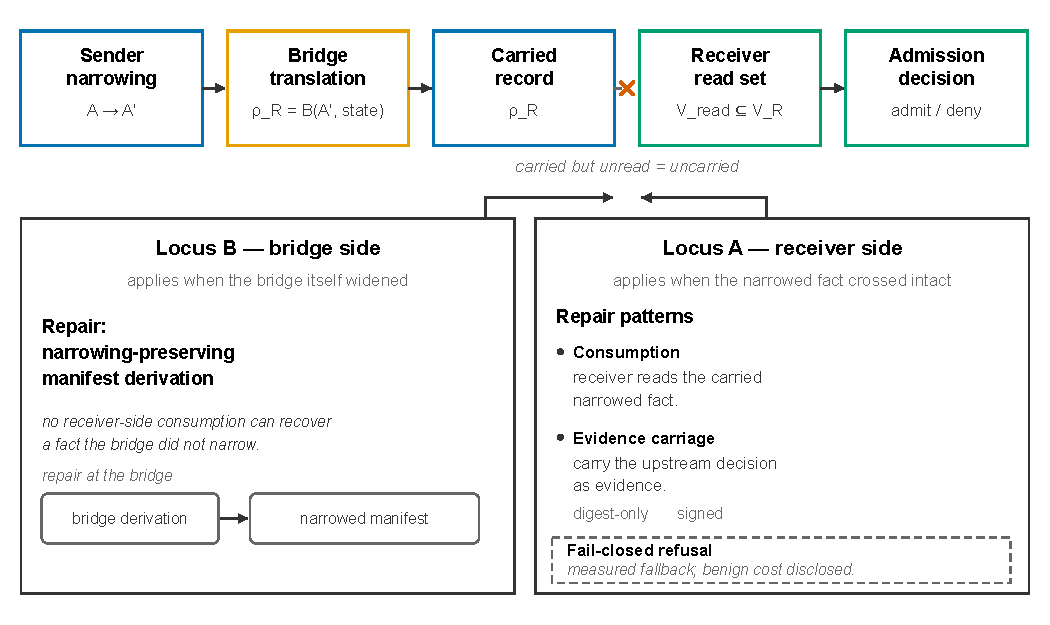
\includegraphics[width=\linewidth,height=\textheight,keepaspectratio,alt={Figure
2. Where the decision can be rescued --- the two repair loci of the seam
program (schematic; no data). The upper band traces one delegated call
through the pipeline these runs instrument: sender narrowing, bridge
translation, the carried record, the receiver's read set, and the
admission decision. Locus A sits at the receiver's admission step and
applies when the narrowed fact crossed intact: evidence carriage of the
upstream decision (digest-only in Pilot 1; signed in the SentinelAgent
pair and E1 M2-auth), with the fail-closed refusal drawn as the measured
fallback and its benign cost disclosed. Locus B sits at the bridge's
derivation step and applies when the bridge did not carry the narrowed
fact into the receiver's contract: the extension's mini-run shows that a
receiver-side check reading snapshot.actions before synthesis reproduces
the decision of the missing derivation (the lock records it as
decision-equivalent to restricting the contract's MAY set), and the
boundary requires a narrowing-preserving manifest derivation, since no
receiver-side consumption can recover a fact the bridge did not narrow.
The annotation carried but unread = uncarried labels the gap between the
carried record and the receiver's read set; Locus B points to the
bridge-translation step, and Locus A points to that gap. Content is
definitional-plus-measured (Section 3.2; the measured repair instances
above); the figure carries no numbers and asserts no
statuses.}]{figures/figure_2_repair_loci.pdf}
\caption{\textbf{Figure 2.} Where the decision can be rescued --- the
two repair loci of the seam program (schematic; no data). The upper band
traces one delegated call through the pipeline these runs instrument:
sender narrowing, bridge translation, the carried record, the receiver's
read set, and the admission decision. Locus A sits at the receiver's
admission step and applies when the narrowed fact crossed intact:
evidence carriage of the upstream decision (digest-only in Pilot 1;
signed in the SentinelAgent pair and E1 M2-auth), with the fail-closed
refusal drawn as the measured fallback and its benign cost disclosed.
Locus B sits at the bridge's derivation step and applies when the bridge
did not carry the narrowed fact into the receiver's contract: the
extension's mini-run shows that a receiver-side check reading
\protect\texttt{snapshot.actions} before synthesis reproduces the
decision of the missing derivation (the lock records it as
decision-equivalent to restricting the contract's MAY set), and the
boundary requires a narrowing-preserving manifest derivation, since no
receiver-side consumption can recover a fact the bridge did not narrow.
The annotation \protect\texttt{carried\ but\ unread\ =\ uncarried}
labels the gap between the carried record and the receiver's read set;
Locus B points to the bridge-translation step, and Locus A points to
that gap. Content is definitional-plus-measured (Section 3.2; the
measured repair instances above); the figure carries no numbers and
asserts no statuses.}\label{fig:figure2}
\end{figure}

No unconditional reading is available from these runs, and each sentence
above is bounded the way its evidence is: by its scoring convention, by
its case set, and by the trust model of the arm it describes. The
two-count reading is the paper's main methodological correction: a zero
in receiver-relative novelty is not a zero in sender-relative violation,
and the difference is where the repair question lives.

\section{5. Discussion --- when seams add authority; repair
patterns}\label{discussion-when-seams-add-authority-repair-patterns}

\textbf{The practical question.} This section answers two questions the
program was built to answer: when does a composed arm admit a call the
sender's narrowing denies, and when does composition add an admission
beyond what the standalone receiver already exhibits? The anatomy is the
familiar one: a sender narrows authority, a bridge translates the
narrowed decision plus state into a receiver-side record, and the
receiver decides from that record. No party owns the seam. The measured
answer is bounded: the one family that can look composition-specific is
E1 under arm-native scoring, but it is an illustration of scoring
dependence rather than a result --- arms 2 and 5 decide identically on
all eight E1 cases and their contracts are byte-identical --- and the
rest is the frozen case sets. The sender-relative violations are broader
(24/40 and 28/48) but are not composition-specific. It is not a general
claim about seams, and no production-safety claim is made for any repair
arm. Every positive sentence below is conditional on the frozen
mappings, case sets, and scoring conventions.

\textbf{Where the composed arm alone admits.} On the E1 action family,
under arm-native scoring, the receiver-relative count exists only in the
composed arm; the recorded admission decisions do not differ. Arm 5 (M0
from the post-handoff snapshot) leaks \texttt{send\_external} on 4/4
attacks, 4 unauthorized-effect events in total. Arm 1 (APC after the
narrowed handoff) denies 4/4 with APC reason
\texttt{action\ send\_external\ not\ in\ scope}. Arm 6 (M2-auth signed
evidence) denies 4/4 with \texttt{PROOF-GAP}, and all 8 signed records
verify \texttt{EVIDENCE-VERIFIED} (report-only; Section 4.2). Arm 7
(shadow denial retained) denies 4/4. Benign calls are allowed 4/4 in
every arm, zero false denials.

The attributable locus is the bridge's contract construction: arm 5's
snapshot carries the narrowed action set
\texttt{actions\ =\ {[}read\_public,\ save\_internal{]}}, but the bridge
builds the receiver's contract from the requested tool, so the contract
never carries the narrowed set. The receiver is not declining to read a
carried fact; the fact is not carried into its contract. Under the
frozen family-wide convention, the arm-2 and arm-5 leaked sets are
identical. Under arm-native scoring, arm 2 is scored safe and that
identity no longer holds. The family-wide identity is forced by
construction and carries no evidential weight about composition. It is
disclosed as a convention, not evidence. This is a bridge-construction
instance of the seam, not the blindness observation's measured instance:
the snapshot carried the narrowed set, the contract did not, and the
failure is located in the bridge, not in the receiver's read set.

\textbf{A scoring-dependent illustration on one family.} Under
arm-native scoring on both arms (each arm scored by the authority its
own world confers), arm 2 is re-scored safe on all 4 attacks and arm 5
leaks 4/4, so the receiver-relative count is 4/4. The recorded decisions
are identical, however: both arms allow all eight cases, and the 4/4
count is produced by re-scoring arm 2 under a norm locked at
\texttt{2026-10-19T12:52:51Z}, after the E1 run began at
\texttt{2026-10-19T07:12:26Z}. Under the frozen family-wide convention
the same records give 0/4 receiver-relative novelty. The sender-relative
count is 4/4 under both. The difference is the scoring convention
applied to identical records, and that dependence is disclosed. Test 1
(scoring-only re-analysis, zero new executions) showed arm 2 safe
against its own world's root authority (0/4 leaks under the root norm)
while the frozen handoff-norm scoring kept the 4 leaks. The
receiver-relative count is 4/4 under arm-native scoring and 0 under the
family-wide convention.

Test 2 resolves the repair locus with execution: an M0-A admission rule
that reads \texttt{snapshot.actions} before synthesis denies all 4
attacks with gate code \texttt{ACTION-SCOPE}, allows all 4 benign cases,
verifies 12/12 receipts, and leaves the arm-2 control unchanged: 8/8
gate-outcome parity, 8/8 byte-identical contract digests, 10/10 locked
predictions matched. The variant does not alter contract synthesis; it
calls canonical M0 unchanged after the check, and the lock records the
check as decision-equivalent to restricting the contract's MAY set to
\texttt{snapshot.actions}. The measured repair is receiver-side
consumption of the snapshot fact; the contract-level form was not
separately executed. It is not evidence that the unmodified receiver
read a fact its contract carried, because the contract did not contain
the set. The \texttt{ACTION-SCOPE-ABSENT} fail-closed branch (missing or
empty action field) was not exercised in this family because every
snapshot carries a non-empty action set. It remains untested here.

\textbf{Repairs.} Four loci follow: three receiver-side (evidence
carriage, retain the upstream denial, action-scope consumption), plus
the derivation-side rule from Section 3.2 (Figure 2). Action-scope
consumption can also be implemented at the bridge by restricting the
synthesized contract's MAY set, which the lock records as
decision-equivalent; Test 2 measured the pre-synthesis form.

\emph{Evidence carriage (receiver).} When the upstream decision can be
carried as evidence, carrying it closes the measured leaks. In the
SentinelAgent pair, arm 6 (signed attestation) closes all 28 baseline
leaks with 0 leaks and 0 false denials. In E1, arm 6 (M2-auth) carries
the upstream denial as signed evidence and denies 4/4 attacks; all 8
signed records verify \texttt{EVIDENCE-VERIFIED} (report-only). In Pilot
1, arm 6 carries the decision as a digest-only record and closes the
24/40 baseline leaks. The caveat is load-bearing: the signed arms assume
the attestation is verified under the trusted key, and M2-auth narrows
tamper and replay but does not establish authenticated transport --- the
signer is the same harness that was the original trust anchor, and any
holder of the public test key can mint valid records. Evidence carriage
is therefore a fix only relative to a correctly deciding upstream: had
the upstream APC admitted a widened scope, M2 would admit it too.

\emph{Retain the upstream denial (receiver).} Keeping the sender's
denial closes leaks at a measured utility cost. Pilot 1 arm 7
(fail-closed): 0 leaks on 40 attack cases, 20/40 benign false-denial
cases, 28 false-denial events. SA arm 7: 0 leaks, 20 benign false-denial
cases, 28 false-denial events. Boundary arm 7 (fail-closed): 0 leaks,
SHADOW-DENY on the 4 seam cases per variant, 20 benign FD cases / 28 FD
events. The utility cost is real: legitimate benign tasks are refused,
and the cost is measured rather than asserted. Neither arm 6 nor arm 7
is production-safe; both are scoped design choices.

\emph{Action-scope consumption (receiver; contract-level equivalent at
the bridge).} Merely carrying the fact in the snapshot without reading
it does not enforce. E1 Test 2 adds an admission check that reads
\texttt{snapshot.actions} before synthesis: 4/4 attacks denied on
\texttt{ACTION-SCOPE}, 4/4 benign allowed, 0 false denials, arm-2
control unchanged. The variant leaves contract synthesis unchanged, and
the lock records the check as decision-equivalent to restricting the
contract's MAY set to \texttt{snapshot.actions}; the contract-level form
was not separately executed. The measured repair is receiver-side
consumption, and it is not evidence that the unmodified receiver ignored
a fact its contract carried. The rule as implemented denies when the
action snapshot is absent or empty (fail-closed), denies when the
requested tool is outside the carried action set, and otherwise runs the
unchanged synthesis.

\emph{Derivation-side narrowing-preserving meet (bridge).} When the
bridge itself widened the manifest (V1/V2), no receiver-side rule can
recover a fact never narrowed. Boundary arm 5 leaks 32 cases / 34
events, which decompose as 28 pre-existing canonical leaks plus the 4
new cases per variant (32 = 28 + 4); standalone arm 2v leaks the
identical 4 per variant; canonical arm 2 is safe on the variant-specific
cases; arms 6/7 suppress APC-DENY / SHADOW-DENY ×4 per variant; seam
count 4 per variant. Composition neither creates nor removes the
failure: the identical admissions appear standalone in the variant arm.
The fault is the bridge's manifest derivation --- V1 widens role scope
beyond root R, V2 default-fills the SEND endpoint --- so the repair
belongs at the bridge, not the receiver. Fix the derivation at the
bridge.

\textbf{Keyholder finding (H5).} Signature verification attests key
possession and payload integrity, not who minted the record; any
keyholder is equivalent to the issuer within the token vocabulary. This
holds for delegate-minted tokens --- \texttt{keyholder\_widen} admitted
4/4 in arms 2/5 --- and for the bridge's own manifest derivation
(V1/V2). SA signature controls: 4 \texttt{SIGNATURE\_INVALID} per token
arm for foreign-key probes; all 10 controls passed. Key distribution is
the seam's critical interface: integrity plus key possession is not
source of authority, so trusting a signature is not the same as trusting
the minter.

\textbf{Positioning.} This paper offers two deliverables: a replication
package and a repair taxonomy. The package contains the frozen case
sets, harnesses, locks, and the locked-prediction protocol so that an
independent reader can re-run the measurements; it is a release
candidate, not a conformance service, certification, or benchmark, and
it reports what a mapping carries rather than fixing it. The design rule
is narrowing preservation at the mapping layer, with the measured
receiver-locus repair (evidence carriage) applied when the upstream
decision reaches the receiver, action-scope consumption when the
narrowed set is present but unread (E1 Test 2, decision-equivalent to
restricting the contract's MAY set), and the derivation-side fix when
the bridge widened the manifest. A broader expansion is a post-workshop
decision, never a commitment made here. No roadmap; no production-safety
claim.

\textbf{Statuses.} H1 \texttt{REFINED}; H2 \texttt{SUPPORTED}; H3
\texttt{REFINED}; H5 \texttt{REFINED}; H6 \texttt{REFINED}; ★
\texttt{REFINED}.

\textbf{Disclosures.} Receiver-relative novelty zero holds only for
narrowing-preserving mappings (canonical T0) on the frozen case sets,
with the E1 scoring illustration and the bridge artifacts disclosed.
Sender-relative violations are 24/40 and 28/48 and are not zero. The two
pair-pilot zeroes are construction-forced; E1 is an illustration of
scoring dependence, not a composition-specific test: arms 2 and 5 decide
identically and their contracts are byte-identical, the 4/4 novelty is
scoring-dependent (family-wide 0/4 vs arm-native 4/4), and the
arm-native norm was recorded after the E1 records existed. The E1
illustration is one family, 1 design point × 4, with the widening-only
operationalization caveat. H1's resource clause is not supported (the
locked C1a prediction was falsified on 4/4 cases); H3 is field-level; H6
pair similarity is partly construction-forced. Arm 6 assumes attestation
verified under the trusted key; arm 7 accepts 20 benign false denials;
neither arm is production-safe; M2-auth does not establish authenticated
transport. No claims beyond the frozen sets.

Table 15 collects the repair loci with their measured results.

\textbf{Table 15.} Repair patterns --- four repair loci with measured
results.

{\def\LTcaptype{none} % do not increment counter
\begin{longtable}[]{@{}
  >{\raggedright\arraybackslash}p{(\linewidth - 4\tabcolsep) * \real{0.1600}}
  >{\raggedright\arraybackslash}p{(\linewidth - 4\tabcolsep) * \real{0.3400}}
  >{\raggedright\arraybackslash}p{(\linewidth - 4\tabcolsep) * \real{0.5000}}@{}}
\toprule\noalign{}
\begin{minipage}[b]{\linewidth}\raggedright
Repair locus
\end{minipage} & \begin{minipage}[b]{\linewidth}\raggedright
Repair
\end{minipage} & \begin{minipage}[b]{\linewidth}\raggedright
Measured result
\end{minipage} \\
\midrule\noalign{}
\endhead
\bottomrule\noalign{}
\endlastfoot
(a) receiver-side evidence carriage & carry upstream decision as
evidence (digest-only in Pilot 1; signed in SA and E1 M2-auth) & Pilot 1
arm 6: 0 leaks (24/40 baseline closed), 0 false denials; SA arm 6: 0
leaks (all 28 baseline leaks closed), 0 false denials; E1 arm 6 M2-auth:
4/4 denied (8/8 signed records \texttt{EVIDENCE-VERIFIED},
report-only) \\
(b) receiver-side retain the upstream denial & retain upstream denial
(fail-closed / shadow deny) & Pilot 1 arm 7: 0 leaks; 20 benign FD
cases; 28 FD events; SA arm 7: 0 leaks; 20 benign FD cases / 28 FD
events; boundary arm 7: 0 leaks; SHADOW-DENY ×4 per variant; 20 benign
FD / 28 FD events \\
(c) receiver-side action-scope consumption (contract-level equivalent at
the bridge) & read \texttt{snapshot.actions} before admission; the lock
records this as decision-equivalent to restricting the contract's MAY
set & E1 Test 2: 4/4 attacks denied \texttt{ACTION-SCOPE}; 4/4 benign
allowed; 12/12 receipts; arm-2 parity 8/8, digests 8/8; 10/10
predictions \\
derivation-side rule & narrowing-preserving meet at bridge & Boundary
arm 5: 32 cases / 34 events = 28 pre-existing + 4 new per variant (32 =
28 + 4); standalone arm 2v leaks identical 4 per variant; seam count 4
per variant \\
\end{longtable}
}

\section{6. Related work}\label{related-work}

\textbf{Purpose.} This section positions the work against four bodies of
literature: the three upstream approaches' own guarantees, as already
reported in Section 2 and not re-measured here; the standards and
authorization systems that supply the vocabulary of attenuation,
evidence, and relationship-based policy; the 2026 agent-delegation line
that proposes compositional authorization for agents; and the
industry/standards pointers carried from the frozen claim set. It also
discusses two close related works, Progent and MasDrift. The section
reports no new results, and guard language applies to others' numbers
throughout. There are no tables and no figures in this section.

\textbf{Upstream formal spines.} APC's ``Composition Soundness'' (Thm
4.7) is intra-session composition of action sequences, conditional on a
complete effective restriction set, serialized admission, and static X
--- a within-mechanism guarantee, not a cross-mechanism composition
guarantee. TraceGrant's Eq. 10 is a contract-soundness assumption,
assessed empirically in its §5.4, not proved. SentinelAgent's Thm 4 is
composition safety for two chains that both satisfy P1--P7 within its
own framework; it does not cover a chain handed to a different
mechanism's decision procedure. Each guarantee stops at its own
boundary. This paper's narrowing-preservation rule plus the blindness
observation (Section 3.2) addresses the question the three guarantees
leave open: the moment authority crosses from one mechanism's vocabulary
into another's. No upstream mechanism is claimed broken or failing; all
upstream figures remain their authors' self-reports, and ``reports'' is
the operative word, never ``achieves''.

\textbf{Industry / standards landscape.} These are pointers only; their
bibliographic identities were checked, but their claims are unverified
and none is treated as a verified fact. Noma {[}Noma{]} (Apr 2026) is
cited as an adjacent industry framing of inter-agent trust at handoffs;
the IETF draft {[}IETF-AuthZ{]} (revised Aug 2026) is cited as a related
cross-domain authorization-sharing proposal. Neither is a measurement of
the specific cross-mechanism translation gap this program instruments,
and neither is adopted here as a result or a fix. Tallam {[}Tallam{]} is
an academic preprint cited as a related reference in the same area. None
of these is a benchmark, a reproduced result, or a verified input to
this manuscript; each citation is a pointer whose claims were not
reproduced, and the frozen claim set governs if any pointer differs from
it.

\textbf{Standards and credential vocabularies.} RFC 8693 {[}RFC8693{]}
defines OAuth 2.0 token exchange, including delegation and impersonation
semantics for security tokens; RFC 9396 {[}RFC9396{]} defines rich
authorization requests, which carry fine-grained authorization data as
structured \texttt{authorization\_details}. Together they standardize
how authority is requested and exchanged across domains, but neither
specifies whether a receiver's admission reads the narrowed fact after
the exchange. Macaroons {[}Macaroons{]} make attenuation explicit
through contextual caveats, and RFC 2693 {[}SPKI{]} gives the theory
behind SPKI certificates and ACLs, including certificate chains. These
are the established vocabularies for expressing, attenuating, and
certifying authority; the seam measured here is the translation step
between such a credential and a heterogeneous receiver's local decision.
They are cited for definitions and contrast only, not as baselines.

\textbf{Systems and foundations.} Miller's {[}Miller{]}
object-capability analysis treats composition and confinement as
properties of how authority is held and passed; Blaze, Feigenbaum, and
Lacy {[}Blaze{]} frame trust management as the joint evaluation of
policy, credentials, and trust; Appel and Felten's {[}Appel{]}
proof-carrying authentication makes the client carry evidence that the
server checks before admission. Fong's {[}Fong{]} relationship-based
access control derives decisions from relationships and policy, and
Zanzibar {[}Zanzibar{]} evaluates relationship tuples against a
consistent, global authorization graph. These lines answer how to
express, confine, attest, or derive authority. This paper asks a
narrower question: whether a cross-mechanism handoff consumes the facts
that carry the narrowing. None is re-implemented, reproduced, or used as
a baseline.

\textbf{Recent agent-delegation work.} A 2026 line proposes
compositional authorization and delegation mechanisms for agents. The
least-autonomy theory of Parisel {[}Parisel{]} argues that per-action
permission bounds are insufficient when actions can be combined, and
formalizes a compositional blast radius and a collusion predicate over
an agent influence graph. ChainCaps {[}ChainCaps{]} enforces monotonic
capability attenuation across tool composition and names permission
laundering as the failure mode. Overlaying Governance {[}Overlaying{]}
supplies a compositional delegation-and-scope framework that overlays
agentic semantics onto relational policies. Local Allow, Global Deny
{[}Pandey{]} proves that per-action authorization does not compose for
relational \emph{purpose} violations, characterizing them as 2-safety
hyperproperties that no per-action monitor which never raises false
alarms can detect. These works propose theories, mechanisms, frameworks,
or impossibility results. None reports a cross-mechanism measurement of
whether a heterogeneous receiver's admission reads the narrowed fact,
which is the question here. They are positioning anchors, not baselines;
no number is compared, and no novelty claim is made over them.

\textbf{Progent (reference only).} Progent is cited as a close related
work on monotonic confinement inside a single privilege-control layer.
No Progent figure is reproduced, re-measured, or compared here; the
paper uses no Progent number as evidence, and no Progent result is
treated as an input or a baseline. The word is ``reports,'' never
``achieves''; Progent is cited as a reference only.

\textbf{MasDrift (related work).} MasDrift studies authorization
preservation across multi-agent coordination architectures using benign
productivity tasks, and its defense propagates an attenuated policy
along the agent chain {[}MasDrift{]}. The narrower question here
concerns executions through two specific public authorization artifacts
and their argument-binding paths, and whether the receiving admission
consumes the narrowing after the chain hands off; the small
deterministic matrix is a conformance study, not an architecture
benchmark and not a substitute for MasDrift's broader evaluation. No
MasDrift number is reproduced, re-measured, or compared.

\textbf{Disclosures.} Others' numbers stay self-reported. Nothing claims
APC, TraceGrant, SentinelAgent, Progent, or MasDrift is broken or fails;
no vulnerability in any upstream mechanism as published is claimed. No
production-safety claim; no benchmark comparability. No claim in this
section upgrades an external work into a measured input, a baseline, or
a result of this program. The industry/standards pointer set (Noma
{[}Noma{]} and the IETF draft {[}IETF-AuthZ{]}) is described as
pointers, not verified facts; Tallam {[}Tallam{]} is an academic
preprint, also not a verified input. The standards, systems, and 2026
agent-delegation anchors are cited for definitions, contrast, and
positioning only; none is a baseline, a reproduced result, or a verified
input. No result in this paper depends on any of their claims.

\textbf{Scope of positioning.} The reference list is a positioning
sample, not a survey: it covers the three measured formal spines, the
standards and systems that define the relevant vocabulary, the closest
2026 agent-delegation work, the two nearest empirical relatives, and the
industry pointers already in the frozen claim set. It does not attempt a
comprehensive survey of delegation, capability, or policy literature,
and the paper does not assert novelty over work outside this positioning
sample. A comparative treatment against any of these systems would
require running it under a common lock with the same case families; none
is run here, and none of their numbers is reproduced.

\section{7. Threats to validity}\label{threats-to-validity}

This section states what the measured program does not claim: the
construct limits of the case sets, the internal limits of the
reconciliation record, and the external limits of interpretation. Two
hypotheses remain open as future instruments; every other limitation is
a plain disclosure, not a softened claim. Table 18 maps each threat to
the section that raises it.

\subsection{7.1 Construct threats}\label{construct-threats}

The case sets are constructed witnesses, not benchmarks. The first pilot
family is 10 templates × 8 runs and the SentinelAgent family is 12
templates × 8 runs, each written for this program and frozen before any
run. Their structure, not their scale, is what licenses a reading: the
E1 extension rests on a single design point with a neutralized parameter
axis, measured as 1 design point × 4 attack cases, and the boundary run
rests on two design points, each 1 × 4 cases --- 8 attack cases in
total, which are not 8 independent cases.

Convention dependence is a construct threat as much as a disclosure. The
E1 receiver-relative count is 0/4 under the frozen family-wide
convention and 4/4 under the arm-native convention. The sender-relative
count is 4/4 under both. The convention is disclosed, and the arm-native
norm was recorded after the E1 records existed (Section 4.2); arms 2 and
5 make identical decisions and their contracts are byte-identical, so
the count difference is a re-scoring, not a behavioural difference.
SentinelAgent scoring is arm-invariant, and rescoping it would flip
\texttt{composition\_history\_loss} arm 2 from leak to safe. At the
boundary, arm 2 is always canonical regardless of the variant loop
variable while the variant arms use the variant manifest derivation, so
the identity of arm 2v with arm 5 per variant is forced by construction.
The composed arm's absolute count is accordingly 32 = 28 + 4: the
pre-existing canonical set plus the per-variant new cases. Three forced
identities are identities of leak sets, not claims that every case
leaks: Pilot 1 arm 2 ≡ arm 5 at 24/24 leaked cases and 26/26 events,
SentinelAgent arm 2 ≡ arm 5 at 28/28 leaked cases, and boundary arm 2v ≡
arm 5 at 32/32 leaked cases per variant. They carry no evidential weight
about composition and are labeled forced.

Two operational caveats complete the construct picture. As
operationalized, the E1 seam test can fire only where the composition
widens: a zero where it does not does not by itself establish
composition-independence, and the same caveat may attach to the original
pilots' seam test, which was not re-verified on that point. Separately,
arm 2's authority assignment in E1 is a disclosed convention --- the
own-world norm is the one discriminating Test 1 adopts, and under the
alternative reading the same records locate the failure in the mapping's
authority assignment, still not in a mechanism interaction. The
field-level audit in Table 13 is limited to the fields exercised by the
frozen templates; it is not a complete inventory of either mechanism.

\subsection{7.2 Internal threats}\label{internal-threats}

The reconciliation record is part of the evidence and was never edited.
Within the SentinelAgent reconciliation, the two checks that failed are
recorded verbatim: false-denial events locked as 26 and observed as 28,
and the arm-5 confusion true-negative denominator locked as 68 and
observed as 20 on the attack-case basis. Both carry
\texttt{affects\_behavior\_cells:\ false} in that record, which is why
they change no outcome cell and remain on file. At the boundary, the
reconciliation records \texttt{expected\_vs\_observed\_ok} as a scope
check --- it verifies the manifest's expected seam count and nothing
beyond it --- and the canonical arm-2 leak scope was carried as
overstated: 0 in the locked reading against 28 pre-existing observed
cases.

\textbf{Deviations from the pre-run plan.} Table 16 lists the
commitments that were not met, the scoring choices made after a run, and
the disposition of each. Table 17 gives the eight boundary-lock cells
that failed, cell by cell.

\textbf{Table 16.} Pre-run commitments, observed deviations, and
dispositions.

{\def\LTcaptype{none} % do not increment counter
\begin{longtable}[]{@{}
  >{\raggedright\arraybackslash}p{(\linewidth - 6\tabcolsep) * \real{0.1500}}
  >{\raggedright\arraybackslash}p{(\linewidth - 6\tabcolsep) * \real{0.3300}}
  >{\raggedright\arraybackslash}p{(\linewidth - 6\tabcolsep) * \real{0.3200}}
  >{\raggedright\arraybackslash}p{(\linewidth - 6\tabcolsep) * \real{0.2000}}@{}}
\toprule\noalign{}
\begin{minipage}[b]{\linewidth}\raggedright
Commitment
\end{minipage} & \begin{minipage}[b]{\linewidth}\raggedright
What was promised or assumed
\end{minipage} & \begin{minipage}[b]{\linewidth}\raggedright
What was observed
\end{minipage} & \begin{minipage}[b]{\linewidth}\raggedright
Disclosure and disposition
\end{minipage} \\
\midrule\noalign{}
\endhead
\bottomrule\noalign{}
\endlastfoot
M3 task-level Contract diagnostic &
\texttt{call\_to\_contract\_mapping.md} §7 promises an M3 diagnostic,
with results reported separately & Not implemented; no M3 code in the
adapters or \texttt{run\_v2.py}; no M3 result exists & Disclosed here;
no M3 result is claimed, and the omission is not repaired
retrospectively \\
§10 classification rule & Mapping document §10 commits to trying
M1/M2/M3 alternatives before a finding is kept & E1's central verdict
was recorded without M3 or an action-scope alternative; Test 2 later ran
an additional M0-A variant, not the M3 diagnostic named in §7, so the
§10 sequence is not satisfied & E1 is reclassified in this revision as a
bridge-construction and scoring illustration, not a composition-specific
result \\
Pilot-1 stop rule & \texttt{STOP\_OR\_CONTINUE.md:41-43}: continue to a
second mechanism pair only if the authenticated-evidence follow-up
produces a failure not attributable to trusted-input assumptions or the
one-step Contract shape & The second pair was run after E1 M2-auth
denied 4/4; it found the same state/identity failure class under a token
bridge, attributable to the same one-step construction, so no qualifying
distinct failure is recorded & The SentinelAgent pair is reported as a
separate construction, not as satisfying the stop rule \\
Boundary lock & 12 per-arm-variant cells (6 arms × 2 variants) with
absolute leak, event, and false-denial predictions & 8 cells failed;
only the arm-2 canonical overstatement was carried into
\texttt{reconciliation.json} & All 8 are listed in Table 17; outcome
cells and variant-specific claims are unchanged \\
SentinelAgent predictions & 96 case predictions locked at
\texttt{2026-10-19T11:52:24Z} & 8 overrides (four
\texttt{resource\_widen}, four \texttt{unsatisfiable\_verify}) flip
unsafe to safe; Pilot 1 completed at \texttt{06:35:32Z}, before the lock
& Case-level leak-set accuracy with the overrides is 96/96; without
them, 8 of 48 attack predictions fail. Disclosed in Section 4.3 \\
E1 scoring norm & The frozen family-wide convention is the primary
reference & The arm-native norm was recorded at
\texttt{2026-10-19T12:52:51Z}; the E1 run started at \texttt{07:12:26Z}
& E1's 4/4 count is reported as scoring-dependent, not as a
pre-registered result \\
Progent receiver & The design space names Progent as a reference
receiver candidate & No Progent run, trace, or metrics file is present
in the frozen artifact tree; a Progent wrapper is vendored only & No
Progent result is reported or claimed in this manuscript \\
\end{longtable}
}

\textbf{Table 17.} Boundary lock: the eight failed per-arm-variant
cells. Each row is one locked cell; the observed value is the value in
\path{b\metrics.json}; the lock is in
\path{design\boundary_lock.json}.

{\def\LTcaptype{none} % do not increment counter
\begin{longtable}[]{@{}
  >{\raggedright\arraybackslash}p{(\linewidth - 6\tabcolsep) * \real{0.4000}}
  >{\raggedright\arraybackslash}p{(\linewidth - 6\tabcolsep) * \real{0.3143}}
  >{\raggedright\arraybackslash}p{(\linewidth - 6\tabcolsep) * \real{0.1429}}
  >{\raggedright\arraybackslash}p{(\linewidth - 6\tabcolsep) * \real{0.1429}}@{}}
\toprule\noalign{}
\begin{minipage}[b]{\linewidth}\raggedright
Arm-variant cell
\end{minipage} & \begin{minipage}[b]{\linewidth}\raggedright
Metric
\end{minipage} & \begin{minipage}[b]{\linewidth}\raggedright
Locked
\end{minipage} & \begin{minipage}[b]{\linewidth}\raggedright
Observed
\end{minipage} \\
\midrule\noalign{}
\endhead
\bottomrule\noalign{}
\endlastfoot
\texttt{sentinelagent\_alone::v1} & leak cases & 0 & 28 \\
\texttt{sentinelagent\_alone::v2} & leak cases & 0 & 28 \\
\texttt{apc\_sentinelagent\_scope\_only::v1} & leak cases & 4 & 32 \\
\texttt{apc\_sentinelagent\_scope\_only::v2} & leak cases & 4 & 32 \\
\texttt{sentinelagent\_alone\_variant::v1} & leak cases & 4 & 32 \\
\texttt{sentinelagent\_alone\_variant::v2} & leak cases & 4 & 32 \\
\texttt{apc\_sentinelagent\_fail\_closed::v1} & false-denial events & 0
& 28 \\
\texttt{apc\_sentinelagent\_fail\_closed::v2} & false-denial events & 0
& 28 \\
\end{longtable}
}

\emph{Note:} the 28 pre-existing leaks in the canonical arm are the
state/identity and signature-family leaks already reported in Section
4.3; the variant-specific four are the boundary's new cases. The lock's
absolute per-cell predictions were not met; the variant-specific
contrast (arm 2 safe on the four variant cases, arm 5 leaks them, arm 2v
leaks them standalone) was met and is the basis of the boundary claim.

Two constraints limit the repair results from inside. Arm 7's
shadow-denial action rule (\texttt{tool\ not\ in\ snapshot.actions}) was
not independently exercised: the retained shadow denial fired first in
all four E1 attacks. And M2-auth does not establish authenticated
transport --- the key is a public test constant, the signer is the same
harness that was the original trust anchor, and there is no forger
control. On the trust side, arm 6 assumes the attestation is verified
under the trusted key and arm 7 accepts 20 benign false denials; neither
repair arm is claimed production-safe, and neither should be read as
one. The E1 precision and recall figures are construction-consistent,
not independent estimates: the attack and benign labels are the same
construction that generates the cases.

\subsection{7.3 External threats}\label{external-threats}

V1/V2 are plausible bridge designs; they may be mis-designs, and they
are not asserted to be typical, the only, or the most likely bridges. No
generalization beyond the frozen case sets is claimed. No vulnerability
is claimed in APC, TraceGrant, or SentinelAgent as published: the
measured findings are properties of this implementation under the locked
bridge mappings and key models, and the upstream mechanisms' own
evaluations remain their authors' self-reports; this manuscript reports
those self-reports and assesses none of those systems. No comparability
with published benchmark numbers is claimed, neither theirs against this
program's counts nor this program's against theirs. Finally, the
zero-novelty statement --- composed arms adding no receiver-relative
admission beyond the receiver's own, under narrowing-preserving mappings
(canonical T0) on the frozen case sets, with the E1 scoring illustration
and the bridge artifacts disclosed as measured --- has the standing of a
recorded property of every case built, not a theorem. Sender-relative
violations are not zero: the composed arms admit 24/40 and 28/48 calls
the sender's narrowing denies in the two pair pilots.

\textbf{Design-space rationale.} The program holds the sender fixed at
APC and varies the receiver across two vocabularies: TraceGrant's
action-scope records and SentinelAgent's state/identity records. That
one-factor design is deliberate. It isolates receiver-side consumption
from sender-specific quirks and keeps the seam test comparable across
pairs. The two receivers were selected for vocabulary contrast and
public availability, not as a representative sample of authorization
mechanisms, and the two bridge variants are this program's own designs.
What travels beyond these cases is the measurement instrument --- the
seam predicate, the two readings, and the repair taxonomy --- not the
measured rates. A different sender, receiver, bridge, or case family
would require its own lock, predictions, and reconciliation; a
production deployment would add transport, key management, and policy
factors that this matrix holds out.

\subsection{7.4 The not-claimed canon}\label{the-not-claimed-canon}

The frozen not-claimed list is restated here by group, without softening
and without upgrading.

Scope of the experiments. Not claimed: bridges beyond V1/V2 --- the two
variants are this program's own constructed designs, and typicality is
not asserted. Not claimed: generalization beyond the frozen case sets,
whose witness sets are as stated in Section 7.1. Not claimed:
comparability with published benchmark numbers, since the case sets are
constructed here and upstream evaluations are self-reported by their
authors. Not claimed: that the zero-novelty result generalizes beyond
these pilots' case families; it is a recorded property of every case
built, not a theorem. Not claimed: that receiver-relative novelty zero
means sender-relative safety --- the sender-relative violations are
reported separately, at 24/40 and 28/48.

Upstream mechanisms. Not claimed: any vulnerability in APC, TraceGrant,
or SentinelAgent as published; the findings are properties of this
implementation under the locked bridge mappings and key models.

Repair patterns. Not claimed: production safety of arms 6 or 7 --- arm 6
assumes the attestation is verified under the trusted key, and arm 7
accepts 20 benign false denials; both are scoped design choices. Not
claimed: authenticated transport for M2-auth --- the key is a public
test constant, the signer is the same harness, and no forger control
exists. Not claimed: arm 7's shadow-denial action rule was independently
exercised --- it was not, because the retained shadow denial fired
first. Not claimed: that the replication package is a conformance
service, certification, or benchmark; it is a release candidate
containing frozen case sets and harnesses.

Conventions. Not claimed: convention-invariance of the seam test --- the
counts differ under frozen family-wide scoring versus arm-native scoring
(0 versus 4/4 for receiver-relative novelty), and the canonical
disclosure is unchanged and remains accurate. Not claimed:
rescoping-neutrality of SentinelAgent scoring, which is arm-invariant
and would flip \texttt{composition\_history\_loss} arm 2 from leak to
safe under rescoping. Not claimed: boundary-convention invariance ---
arm 2 is always canonical regardless of the variant loop variable, and
arm 2v matches arm 5 per variant by construction. Not claimed: that the
seam test as operationalized measures more than where the composition
widens; a zero where it does not would not by itself establish
composition-independence. Not claimed: an unchallenged authority
assignment for arm 2 in E1 --- the own-world norm is a disclosed
convention.

Hypotheses. Not claimed: that H3 is a general law of vocabulary gaps;
the carried claim is the field-level account in Table 13, limited to the
audited fields. Not claimed: that H6 is a general pair-similarity law;
the similarity within the measured pairs is partly construction-forced,
and the E1 action family is an illustration of scoring dependence rather
than a composition-specific result. Not claimed: that H1's resource
clause is false in general; the frozen authority records it as not
supported, because the locked C1a prediction was falsified on 4/4
\texttt{resource\_widen} cases (the cases were predicted unsafe and were
caught), and the case set exercises no resource-side trust failure. Not
claimed: that H3 covers caught representable cases, the E1 action-family
bridge-construction failure, or the V1/V2 derivation widening; those are
reported under H1/H6 and the measured findings, not H3.

Open hypotheses. Not claimed here: the shared-audit-trail hypothesis and
the intent-layer hypothesis --- carried below as unbuilt instruments,
not as findings and not as claims.

\subsection{7.5 Two hypotheses carried
open}\label{two-hypotheses-carried-open}

\textbf{H4 --- \texttt{UNTESTED}.} This is an unmeasured surface, not a
demonstrated failure: H4's claim is that there is no shared audit trail
across the mechanisms --- the SHA-256 evidence chain on the
sender-mechanism side, the receiver's receipts, and the hash-linked
tokens are three separate provenance records, and this hypothesis is not
tested in any pilot. The SentinelAgent tokens in the runs are one-hop,
each parent hash resolving to the root, so no chain reconstruction and
no cross-mechanism trail interchange was exercised in either the
SentinelAgent pilot or the boundary run. The next instrument is
identified but not built here: a case family that reconstructs authority
from a token hash chain and compares it with the APC envelope's history.
Nothing adjacent is imported into this claim.

\textbf{H7 --- \texttt{UNTESTED}.} The intent layer of the SentinelAgent
pair, its principle P2, may be gameable through benign-word override,
and this was not tested: P2's \texttt{intent\_text} was carried in the
run records but never classified, and neither the E1 extension nor the
boundary run exercised it. No probing instrument is introduced in this
paper, and the hypothesis stands as open.

\textbf{H4/H7 gate.} Neither hypothesis was exercised in this revision:
no H4 or H7 experiment was designed, locked, or executed, and no result
for either appears anywhere in this paper. Both remain
\texttt{UNTESTED}; a future test would require a new externally anchored
lock, a case set, and its own reconciliation before it could be
reported. No claim in this paper depends on H4 or H7.

\textbf{Table 18.} Threat ledger - each threat and the section that
raises it.

{\def\LTcaptype{none} % do not increment counter
\begin{longtable}[]{@{}
  >{\raggedright\arraybackslash}p{(\linewidth - 2\tabcolsep) * \real{0.5000}}
  >{\raggedright\arraybackslash}p{(\linewidth - 2\tabcolsep) * \real{0.5000}}@{}}
\toprule\noalign{}
\begin{minipage}[b]{\linewidth}\raggedright
Threat
\end{minipage} & \begin{minipage}[b]{\linewidth}\raggedright
Raised in
\end{minipage} \\
\midrule\noalign{}
\endhead
\bottomrule\noalign{}
\endlastfoot
Bridges beyond V1/V2 out of scope; V1/V2 not asserted typical & Section
7.3 \\
Production safety of the repair arms not claimed & Sections 7.2, 7.4 \\
Shared audit trail and intent layer carried open, not claimed & Section
7.5 \\
Generalization beyond the frozen case sets not claimed & Sections 7.1,
7.4 \\
No vulnerability claim about the upstream mechanisms as published &
Sections 7.3, 7.4 \\
Comparability with published benchmark numbers not claimed & Sections
7.3, 7.4 \\
The zero-novelty result is a recorded property, not a theorem & Sections
7.3, 7.4 \\
Sender-relative violations are not zero; the two readings differ &
Sections 4.5, 7.4 \\
Family-wide versus arm-native convention dependence & Sections 7.1,
7.4 \\
SentinelAgent arm-invariant scoring; rescoping flip & Sections 7.1,
7.4 \\
Boundary arm-2 canonical convention; forced arm-2v identity & Sections
7.1, 7.4 \\
M2-auth does not establish authenticated transport & Sections 7.2,
7.4 \\
Arm 7's shadow-denial action rule not independently exercised & Sections
7.2, 7.4 \\
E1 seam test operationalized only where the composition widens &
Sections 7.1, 7.4 \\
Arm-2 authority assignment as a disclosed convention & Sections 7.1,
7.4 \\
H1 resource clause is not supported (C1a prediction falsified on 4/4
cases) & Sections 4.1, 7.4 \\
H3 is field-level, not a general vocabulary-gap law & Sections 4.3, 4.5,
7.4 \\
H6 pair similarity is partly construction-forced & Sections 4.5, 7.4 \\
E1 precision/recall are construction-consistent, not independent &
Section 7.2 \\
M3 diagnostic, §10 rule, stop-rule continuation, and boundary lock cells
disclosed & Section 7.2 \\
SentinelAgent prediction overrides disclosed with timing and accuracy &
Sections 4.3, 7.2 \\
E1 arm-native norm recorded after the run, not pre-registered & Sections
4.2, 7.1, 7.2 \\
Progent receiver not run in the frozen evidence tree & Section 7.2 \\
Replication package is not a conformance service or certification &
Sections 5, 7.4, 8 \\
\end{longtable}
}

\section{8. Reproducibility and
artifacts}\label{reproducibility-and-artifacts}

This section describes the replication package prepared as a release
candidate --- the program's practical deliverable at workshop stage. It
is protocol description only: what was frozen, what was locked, and what
was re-verified. It carries no result claims, and it is not a
conformance service, certification, or benchmark.

\subsection{8.1 What the package contains and how it was
run}\label{what-the-package-contains-and-how-it-was-run}

The package contains the four frozen experiment sets --- the two pair
pilots, the action-clause extension with its resolving tests and
controls, and the boundary run --- as runnable case sets with their
harnesses under the locked-prediction protocol. Predictions, cases,
arms, and locked input hashes were frozen before execution. The one
recorded harness-hash deviation is Test 2's runner hash, disclosed in
Section 4.2. Executions were strictly sequential, offline, and
deterministic. Discrepancies between predicted and observed values were
reconciled verbatim into files that were never edited after the fact,
and each published number was generated from the artifacts and embedded
byte-verbatim. The execution ledger records the scale: 2,446 = 560 + 40
+ 6 + 16 + 672 + 1,152.

The locks are internally time-stamped, not externally anchored: there is
no registry entry or trusted timestamp, and the repository's git history
begins after the 19 October 2026 runs. ``Pre-registration'' is therefore
reserved for future runs whose locks are anchored externally; this paper
reports an internally time-stamped lock-before-run protocol.

Re-execution discipline is part of the package. The SentinelAgent
program recorded determinism reruns of 20 executions with 0 mismatches,
and its control battery passed 10/10; the boundary run's control battery
passed 7/7. The controls exist so that a reader can check claims about
repair results before trusting them. Scoping limits are carried with the
package as well: there is a single implementation per repair pattern, so
each repair measurement is scoped to its own implementation; the package
reports what a mapping carries and does not fix anything; and
sanitization and cleanup of the release tree remain pending. The package
is a release candidate, not a public release: repository URL, license,
DOI, and archival location are not yet assigned. It is not a conformance
service, certification, or benchmark, and no third party has run it.

\subsection{8.2 The artifact hash
ledger}\label{the-artifact-hash-ledger}

Table 19 lists six frozen addresses; two are also quoted in the text,
and the table is not a complete hash inventory. The numbers in this
paper are traceable through the artifact tree to the artifacts that
generated them. Table 19 transcribes the frozen addresses for the E1
dataset, the discriminating-tests lock, the SentinelAgent lock and case
set, and the boundary lock and harness, in each case from the frozen
source map that records each value and its artifact root.

\textbf{Table 19.} Artifact hash ledger - frozen lock/case/harness
hashes.

{\def\LTcaptype{none} % do not increment counter
\begin{longtable}[]{@{}ll@{}}
\toprule\noalign{}
Artifact & Frozen hash \\
\midrule\noalign{}
\endhead
\bottomrule\noalign{}
\endlastfoot
E1 dataset (canonical \texttt{dataset\_sha256}) &
\texttt{1b7c6083…b2e264ba} \\
Discriminating lock (file SHA-256) & \texttt{8cd4d993…996011ab} \\
SA lock (file SHA-256) & \texttt{9f2611a1…65d47f0} \\
SA cases (file SHA-256) & \texttt{ca2f05d5…e42cb6d2} \\
Boundary lock (file SHA-256) & \texttt{b4deab1a…082c4296} \\
Boundary harness (file SHA-256) & \texttt{fa8f7e42…790814af4} \\
\end{longtable}
}

\emph{Note:} row 1 is the canonical dataset hash recorded in the E1
lock; rows 2--6 are file SHA-256 values. The table is a citation aid,
not a complete hash inventory.

\textbf{Suffix note.} Displayed hashes are variable-length truncations;
row 3 uses a 7-character suffix and row 6 uses a 9-character suffix.
Full 64-character values are in the ancillary \texttt{hashes.txt}.

\textbf{Renumbering note.} The ancillary \texttt{hashes.txt} uses the
pre-renumbering label ``Table 15'' for the six rows presented here as
Table 19. The labels are historical; the values and row order are
unchanged.

\section{9. Conclusion}\label{conclusion}

This paper asked a narrow question about a broad practice: when one
authorization mechanism narrows a decision and hands it to another
through a bridge, what crosses, and what can the receiver no longer
derive? The question matters because the composed pair's decision is
what executes, while each mechanism's own guarantee --- conditional on
its own envelope, its own contracts, its own static assumptions ---
stops at the handoff that nobody owns.

The method was chosen to make the answer auditable rather than merely
reported. Primary predictions, case sets, arms, and hashes were locked
before each run, with later scoring norms and overrides dated and
disclosed; executions were sequential, offline, and deterministic;
mismatches were reconciled verbatim; and every published number was
transcribed and script-checked against the artifacts. Four experiment
sets put 2,446 = 560 + 40 + 6 + 16 + 672 + 1,152 executions behind the
measured statements below.

The measured answer is conditional, and its conditions are part of the
answer. The composed arms commit sender-relative violations on 24/40 and
28/48 attacks in the two pair pilots, but the receiver-only arms admit
the same calls, so receiver-relative novelty is zero; the two pair-pilot
zeroes are construction-forced. The E1 action family illustrates the
limit: the receiver contracts are byte-identical in arms 2 and 5 on all
eight cases, and the 4/4 receiver-relative count appears only under an
arm-native norm recorded after the E1 records existed. It records 4/4
sender-relative violations, 0/4 receiver-relative novelty under the
frozen family-wide convention, 4/4 under arm-native scoring, with an
action-scope rule that reads the snapshot's narrowed set and then denies
4/4 attacks while allowing 4/4 benign calls; the lock records that rule
as decision-equivalent to restricting the contract's MAY set. The
illustration is one design point × four attack cases and is
convention-dependent. At the boundary, two non-narrowing-preserving
bridge designs produced four new cases per variant that appear
identically in the standalone variant arm --- a bridge-design artifact,
not a composition-specific failure. The keyholder caveat stands: a
signature verifies integrity and key possession, not the source of
authority. Every positive sentence here is conditioned on the frozen
sets, the locked mappings, and the scoring conventions under which the
counts were produced.

The practical deliverable is the replication package of Section 8:
frozen case sets, harnesses, and the locked-prediction protocol,
packaged so that an independent reader can re-run the measurements. It
is a release candidate, not a conformance service or certification. The
package reports; it does not fix.

What remains open is stated in Section 7 as unbuilt instruments rather
than findings: no shared audit trail has been measured across the
mechanisms, and the sentinel pair's intent layer has not been probed.
The closing status of the measured program is: H1 \texttt{REFINED}
(action clause measured; resource clause not supported;
manifest-derivation clause measured), H2 \texttt{SUPPORTED}, H3
\texttt{REFINED} (field-level), H5 \texttt{REFINED}, H6
\texttt{REFINED}, and ★ \texttt{REFINED} for the zero-novelty finding
--- with the two open hypotheses above carried forward as instruments,
not claims --- H4 \texttt{UNTESTED}, H7 \texttt{UNTESTED}.

Continuation beyond the workshop decision point is not a commitment made
here; any expansion is a post-workshop decision taken on its own
evidence.

\section{Declarations}\label{declarations}

\textbf{Data availability.} The counts reported here are transcribed and
script-checked against the frozen artifact tree described in Section 8.
The replication package is a release candidate: public archiving is
pending, and no repository URL, DOI, license, or archival location is
asserted because none has been assigned. The frozen case sets,
harnesses, locks, and reconciliation records are retained by the author
and can be made available for inspection on reasonable request, subject
to the release gates in Section 8. No new data were generated for this
revision.

\textbf{Ethics.} No human-subjects data were collected. The experiments
are synthetic and offline, and no personally identifying data were
processed. AI tools assisted with experiment implementation and quality
assurance; Section 3.7 records their roles. No AI system is an author; I
wrote the manuscript and am responsible for all claims, artifacts, and
errors.

\textbf{Author contributions (CRediT).} The manuscript is
single-authored. Prathamesh N Patil is the sole author and performed all
roles: conceptualization, methodology, software, validation, formal
analysis, investigation, data curation, writing (original draft and
review/editing), visualization, and project administration. The author
is responsible for all claims, artifacts, and errors.

\textbf{Competing interests.} The author declares no financial or
non-financial competing interests.

\textbf{Funding.} This research received no external funding.

\textbf{Acknowledgments.} The author thanks the authors of APC and
SentinelAgent for making their published artifacts available for study.

\textbf{Limitations.} The claims are limited to the frozen case sets,
mappings, and scoring conventions in Section 3 and the threats in
Section 7. The case sets are constructed witnesses, not benchmarks; the
E1 illustration is one design point × four attack cases; the boundary
run has two design points; the two pair-pilot zeroes are
construction-forced; and no production-safety or generalization claim is
made. H4 and H7 remain \texttt{UNTESTED}. The replication package is a
release candidate, not a public conformance service.

\section{Appendix A. Hypothesis lineage and
operationalization}\label{appendix-a.-hypothesis-lineage-and-operationalization}

The frozen experiment artifacts predate the current hypothesis key, and
some labels changed meaning between the pilot records and this
manuscript. Table A1 records the lineage so that a legacy label is not
read as the current label with the same number. It is provenance, not
evidence, and it changes no status.

\textbf{Table A1.} Hypothesis lineage --- legacy artifact labels, their
operationalizations, and the current manuscript labels.

{\def\LTcaptype{none} % do not increment counter
\begin{longtable}[]{@{}
  >{\raggedright\arraybackslash}p{(\linewidth - 6\tabcolsep) * \real{0.1800}}
  >{\raggedright\arraybackslash}p{(\linewidth - 6\tabcolsep) * \real{0.3400}}
  >{\raggedright\arraybackslash}p{(\linewidth - 6\tabcolsep) * \real{0.1800}}
  >{\raggedright\arraybackslash}p{(\linewidth - 6\tabcolsep) * \real{0.3000}}@{}}
\toprule\noalign{}
\begin{minipage}[b]{\linewidth}\raggedright
Legacy artifact label
\end{minipage} & \begin{minipage}[b]{\linewidth}\raggedright
Legacy operationalization
\end{minipage} & \begin{minipage}[b]{\linewidth}\raggedright
Current manuscript label
\end{minipage} & \begin{minipage}[b]{\linewidth}\raggedright
Status / provenance
\end{minipage} \\
\midrule\noalign{}
\endhead
\bottomrule\noalign{}
\endlastfoot
H1 (all artifact sets) & Receiving mechanism re-derives scope or trusts
the already-authorized caller & H1 & \texttt{REFINED}; action and
manifest-derivation clauses measured; resource clause not supported (C1a
prediction falsified on 4/4 cases) \\
H2 (all artifact sets) & Dynamic state, identity, and freshness do not
cross and leak & H2 & \texttt{SUPPORTED}; unchanged label \\
H3 (v2 only) & VERIFY postconditions are an admission/completion
boundary & No direct current-H3 equivalent; historical
completion-integrity finding & Reported under H1/H6 and the measured
findings, not current H3. \path{v2\claims_update.md}
H3; \texttt{raw\_metrics.json} \texttt{unsatisfiable\_verify} \\
H4 (v2 only) & Mapping choices decide whether a failure is a mechanism
property or an artifact & No direct current-H4 equivalent; historical
mapping-attribution finding & Reported under H1 \texttt{REFINED} and the
measured findings, not current H4. \texttt{case\_generator.py} tags
recipient/default cases old H4; those are caught-case evidence, not
current H3 or H4 \\
H6 (v2 only) & Comparison with the Progent reference numbers & No
current-H6 equivalent; current H6 is similar-pair vs dissimilar-pair
failure shapes & Historical, directional-only Progent block; not used as
a comparison or baseline. Current H6 rests on the SA/boundary
measurements and is \texttt{REFINED} \\
H3--H6 (SA/boundary) & Vocabulary mismatch; no shared audit trail;
verification gap; similar/dissimilar failure shapes & H3--H6 & H3
\texttt{REFINED} (field-level, Table 13); H4 \texttt{UNTESTED}; H5
\texttt{REFINED}; H6 \texttt{REFINED} \\
H7 (manuscript only) & Intent layer P2 & H7 & \texttt{UNTESTED};
\texttt{intent\_text} carried but never classified \\
\end{longtable}
}

The frozen artifacts are not edited; this table is the reconciliation.
In particular, recipient/default cases tagged old H4 in
\path{tests\seam_pilot_v2\design\case_generator.py}
are caught-case evidence and are not current H3 or current H4 evidence.

\textbf{Status changes from the pre-review draft.} H3 moved from
\texttt{SUPPORTED} to \texttt{REFINED} because the field audit separates
carried-but-unread, read-but-not-carried, and absent, and the broad
vocabulary-gap law is not tested. H6 moved from \texttt{SUPPORTED} to
\texttt{REFINED} because pair similarity is partly construction-forced.
★ moved from \texttt{SUPPORTED} to \texttt{REFINED} because the two
pair-pilot zeroes are forced and E1 is an illustration of scoring
dependence, not a composition-specific test. H1's resource clause
remains not supported in the frozen authority: the locked C1a prediction
was falsified on 4/4 \texttt{resource\_widen} cases, and this manuscript
reports that disposition rather than relabeling it \texttt{UNTESTED}. No
frozen artifact was edited.

\textbf{Table A2.} Effective witness sets behind the reported counts ---
executions, case structure, and independent design points.

{\def\LTcaptype{none} % do not increment counter
\begin{longtable}[]{@{}
  >{\raggedright\arraybackslash}p{(\linewidth - 10\tabcolsep) * \real{0.1327}}
  >{\raggedright\arraybackslash}p{(\linewidth - 10\tabcolsep) * \real{0.1224}}
  >{\raggedright\arraybackslash}p{(\linewidth - 10\tabcolsep) * \real{0.2041}}
  >{\raggedright\arraybackslash}p{(\linewidth - 10\tabcolsep) * \real{0.1224}}
  >{\raggedright\arraybackslash}p{(\linewidth - 10\tabcolsep) * \real{0.2245}}
  >{\raggedright\arraybackslash}p{(\linewidth - 10\tabcolsep) * \real{0.1939}}@{}}
\toprule\noalign{}
\begin{minipage}[b]{\linewidth}\raggedright
Experiment set
\end{minipage} & \begin{minipage}[b]{\linewidth}\raggedright
Executions
\end{minipage} & \begin{minipage}[b]{\linewidth}\raggedright
Cases
\end{minipage} & \begin{minipage}[b]{\linewidth}\raggedright
Attack cases
\end{minipage} & \begin{minipage}[b]{\linewidth}\raggedright
Effective independent witness
\end{minipage} & \begin{minipage}[b]{\linewidth}\raggedright
Construction note
\end{minipage} \\
\midrule\noalign{}
\endhead
\bottomrule\noalign{}
\endlastfoot
Pilot 1 (v2) & 560 & 80 = 10 templates × 8 runs (40 attack + 40 benign)
& 40 = 10 templates × 4 parameters & 6 leak templates × 4 parameters =
24 headline leak cases; one design point per template row & The 24/40
headline counts template cases, not 24 independent designs. \\
E1 extension & 46 = 40 + 6 control & 8 = 4 attack + 4 benign & 4 = 1
design point × 4 cases & 1 design point × 4 attack cases & Recipient and
budget axes neutralized; the four attacks are replicates of one design
point. \\
Discriminating Test 1 & 0 new & 4 frozen arm-2 attack records & 4 & 1
scoring comparison (family-wide versus arm-native) over 4 cases &
Scoring-only re-analysis; no new executions. \\
Discriminating Test 2 & 16 & 8 = 4 attack + 4 benign; 2 arms & 4 = 1
repair design × 4 cases & 1 repair design × 4 attack cases &
Receiver-side action-scope consumption (contract-equivalent); arm-2
control 8/8 gate and digest parity. \\
SentinelAgent pair & 672 & 96 = 12 templates × 8 runs (48 attack + 48
benign) & 48 = 12 templates × 4 parameters & 6 state/identity leak
templates × 4 = 24 of 48; signature family 16 = 2 pairs × 4 document
parameters × 2 variants & The 28/48 headline is 24 state/identity leaks
plus 4 signature-family leaks. \\
Boundary V1/V2 & 1,152 & 96 rows per arm-variant cell; 6 arms × 2
variants & 8 = 2 design points × 4 cases & 1 design point × 4 cases per
variant; 2 design points total & Four new cases per variant; not 8
independent designs. \\
\textbf{Total} & \textbf{2,446 = 560 + 46 + 0 + 16 + 672 + 1,152} & ---
& --- & --- & E1's 46 includes its six control executions, as in Table
3. \\
\end{longtable}
}

\emph{Note:} every cell restates a design fact already stated in
Sections 3.5 and 4.1--4.4; the table introduces no new measurement and
no new count. Executions are matrix runs; the control and replay records
excluded from the 2,446 total remain as stated in Section 3.5.

\textbf{Path notation.} The roots \texttt{v2}, \texttt{dt}, \texttt{sa},
and \texttt{b} are defined in Section 3.5; full paths remain in the
artifact tree.

\section{References}\label{references}

\raggedright

\textbf{{[}APC{]}} Xabier Muruaga. \emph{Bounded Agents: Delegation
Security for Multi-Agent AI Systems.} arXiv:2608.15888v1, 16 August
2026. DOI: 10.48550/arXiv.2608.15888.
\url{https://arxiv.org/abs/2608.15888}. Code:
\url{https://github.com/xmuruaga/bounded-agents} (commit
\texttt{d31a1ea115a3e97ab972ac8d03f23ef36cf9b653}). Theorem 4.7
(Composition Soundness) follows the numbering of the v1 PDF; the arXiv
HTML numbers it 4.8.

\textbf{{[}TraceGrant{]}} Bohao Liao, Jingchao Wang, Qipeng Song, Jin
Cao, Jieling Wang, and Boyu Deng. \emph{TraceGrant: A Contract-Governed
Security Framework for the Task-Effect Lifecycle of Networked LLM
Agents.} arXiv:2608.21126v1, 21 August 2026. DOI:
10.48550/arXiv.2608.21126. \url{https://arxiv.org/abs/2608.21126}.
Contract-governed task-effect authorization, not delegation. No public
code; artifacts are available on reasonable request.

\textbf{{[}SentinelAgent{]}} KrishnaSaiReddy Patil. \emph{SentinelAgent:
Intent-Verified Delegation Chains for Securing Federal Multi-Agent AI
Systems.} arXiv:2604.02767v1, 3 April 2026. DOI:
10.48550/arXiv.2604.02767. \url{https://arxiv.org/abs/2604.02767}.
Prototype: \url{https://github.com/ksrpatil/sentinelagent} (commit
\texttt{b7b1add07b7485e99aa3b91882a3f8f879f2e357}). The upstream
\texttt{sentinelagent\_das\_prototype.py} has SHA-256
\texttt{206a2d5f46d3…} with LF line endings; the \texttt{739d9db1e836…}
hash in the manuscript is of a CRLF-converted copy.

\textbf{{[}Progent{]}} Tianneng Shi, Jingxuan He, Zhun Wang, Hongwei Li,
Linyu Wu, Wenbo Guo, and Dawn Song. \emph{Progent: Securing AI Agents
with Privilege Control.} arXiv:2504.11703v3, revised 14 May 2026. DOI:
10.48550/arXiv.2504.11703. \url{https://arxiv.org/abs/2504.11703}. Code:
\url{https://github.com/sunblaze-ucb/progent}. Versions 1 and 2 were
titled ``Progent: Programmable Privilege Control for LLM Agents''.

\textbf{{[}MasDrift{]}} Zhuoning Xu, Xiucheng Zhang, Hanjun Luo, Yingbin
Jin, Yinpeng Dong, and Hanan Salam. \emph{MasDrift: Benchmarking
Authorization Preservation Across Multi-Agent Architectures.}
arXiv:2608.07556v3, revised 15 October 2026. DOI:
10.48550/arXiv.2608.07556. \url{https://arxiv.org/abs/2608.07556}.

\textbf{{[}Noma{]}} Noma Security. \emph{Your Agents Are Trusting Each
Other - Should They?} Noma Security Blog, 23 April 2026. Byline: Diana
Kelley.
\url{https://noma.security/blog/your-agents-are-trusting-each-other-should-they}.
Industry blog; not peer reviewed.

\textbf{{[}IETF-AuthZ{]}} J. Diaconu, M. Yannuzzi, H. Muyal, F.
Brockners, N. Kale, A. Agarwal, J. Hickman, and A. Lal.
\emph{Cross-Domain AuthZ Information sharing for Agents.} Internet-Draft
draft-diaconu-agents-authz-info-sharing-01, 4 August 2026.
\url{https://datatracker.ietf.org/doc/draft-diaconu-agents-authz-info-sharing/01/}.
Work in progress; not endorsed by the IETF.

\textbf{{[}Tallam{]}} Krti Tallam. \emph{Authorization Propagation in
Multi-Agent AI Systems: Identity Governance as Infrastructure.}
arXiv:2605.05440v1, 6 May 2026. DOI: 10.48550/arXiv.2605.05440.
\url{https://arxiv.org/abs/2605.05440}.

\textbf{{[}RFC8693{]}} M. Jones, A. Nadalin, B. Campbell (Ed.), J.
Bradley, and C. Mortimore. \emph{OAuth 2.0 Token Exchange.} RFC 8693,
Internet Engineering Task Force, January 2020. DOI: 10.17487/RFC8693.
\url{https://www.rfc-editor.org/rfc/rfc8693}. Standards-Track RFC; not a
measurement of this program.

\textbf{{[}Zanzibar{]}} Ruoming Pang, Ramon Caceres, Mike Burrows,
Zhifeng Chen, Pratik Dave, Nathan Germer, Alexander Golynski, Kevin
Graney, Nina Kang, Lea Kissner, Jeffrey L. Korn, Abhishek Parmar,
Christina D. Richards, and Mengzhi Wang. \emph{Zanzibar: Google's
Consistent, Global Authorization System.} 2019 USENIX Annual Technical
Conference (USENIX ATC 19), pp.~33--46, Renton, WA, July 2019.
\url{https://www.usenix.org/conference/atc19/presentation/pang}.
Peer-reviewed conference paper; not reproduced here.

\textbf{{[}Macaroons{]}} Arnar Birgisson, Joe Gibbs Politz, Úlfar
Erlingsson, Ankur Taly, Michael Vrable, and Mark Lentczner.
\emph{Macaroons: Cookies with Contextual Caveats for Decentralized
Authorization in the Cloud.} Network and Distributed System Security
Symposium (NDSS), 2014. DOI: 10.14722/ndss.2014.23212.
\url{https://www.ndss-symposium.org/ndss2014/programme/macaroons-cookies-contextual-caveats-decentralized-authorization-cloud/}.
Peer-reviewed conference paper; not reproduced here.

\textbf{{[}RFC9396{]}} T. Lodderstedt, J. Richer, and B. Campbell.
\emph{OAuth 2.0 Rich Authorization Requests.} RFC 9396, Internet
Engineering Task Force, May 2023. DOI: 10.17487/RFC9396.
\url{https://www.rfc-editor.org/rfc/rfc9396}. Standards-Track RFC; not a
measurement of this program.

\textbf{{[}SPKI{]}} C. Ellison, B. Frantz, B. Lampson, R. Rivest, B.
Thomas, and T. Ylonen. \emph{SPKI Certificate Theory.} RFC 2693,
Internet Engineering Task Force, September 1999. DOI: 10.17487/RFC2693.
\url{https://www.rfc-editor.org/rfc/rfc2693}. Experimental RFC; not a
measurement of this program.

\textbf{{[}Miller{]}} Mark S. Miller. \emph{Robust Composition: Towards
a Unified Approach to Access Control and Concurrency Control.} PhD
thesis, Johns Hopkins University, Baltimore, MD, 2006.
\url{https://jscholarship.library.jhu.edu/items/b8376e55-208e-4fcc-81a2-ad5a7de0acbb}.
No DOI; not reproduced here.

\textbf{{[}Blaze{]}} Matt Blaze, Joan Feigenbaum, and Jack Lacy.
\emph{Decentralized Trust Management.} 1996 IEEE Symposium on Security
and Privacy, pp.~164--173, IEEE Computer Society Press, 1996. DOI:
10.1109/SECPRI.1996.502679. Peer-reviewed conference paper; not
reproduced here.

\textbf{{[}Appel{]}} Andrew W. Appel and Edward W. Felten.
\emph{Proof-Carrying Authentication.} Proceedings of the 6th ACM
Conference on Computer and Communications Security (CCS), pp.~52--62,
ACM, New York, NY, USA, 1999. DOI: 10.1145/319709.319718. Peer-reviewed
conference paper; not reproduced here.

\textbf{{[}Fong{]}} Philip W. L. Fong. \emph{Relationship-Based Access
Control: Protection Model and Policy Language.} Proceedings of the First
ACM Conference on Data and Application Security and Privacy (CODASPY),
pp.~191--202, ACM, New York, NY, USA, 2011. DOI:
10.1145/1943513.1943539. Peer-reviewed conference paper; not reproduced
here.

\textbf{{[}Parisel{]}} Christophe Parisel. \emph{A Theory of Least
Autonomy in AI.} arXiv:2607.09744v1, 3 July 2026. DOI:
10.48550/arXiv.2607.09744. \url{https://arxiv.org/abs/2607.09744}. arXiv
preprint; not reproduced here.

\textbf{{[}ChainCaps{]}} Xiaochong Jiang, Shiqi Yang, Ziwei Li, Lifei
Liu, Haoran Yu, and Yichen Liu. \emph{ChainCaps: Composition-Safe
Tool-Using Agents via Monotonic Capability Attenuation.}
arXiv:2605.26542v4, revised 1 July 2026; presented at the Second
Workshop on Agents in the Wild: Safety, Security, and Beyond (AIWILD) at
ICML 2026 (non-archival). DOI: 10.48550/arXiv.2605.26542.
\url{https://arxiv.org/abs/2605.26542}. Workshop presentation; not
reproduced here.

\textbf{{[}Overlaying{]}} Amjad Ibrahim and Yong Li. \emph{Overlaying
Governance: A Compositional Authorization Framework for Delegation and
Scope in Agentic AI.} arXiv:2606.03518v1, 2 June 2026. DOI:
10.48550/arXiv.2606.03518. \url{https://arxiv.org/abs/2606.03518}. arXiv
preprint; not reproduced here.

\textbf{{[}Pandey{]}} Anmol Pandey, Aditya Jain, Liang Chen, and Carsten
Maple. \emph{Local Allow, Global Deny: Why Per-Action Authorization Does
Not Compose in LLM Agents.} arXiv:2610.27620v1, 20 October 2026;
accepted at the 8th IEEE International Conference on Trust, Privacy and
Security in Intelligent Systems and Applications (IEEE TPS 2026), listed
at \url{https://tps.ieee-cs.org/2026/accepted-papers}.
\url{https://arxiv.org/abs/2610.27620}. Preprint; acceptance listed by
the venue, not independently verified here.

\emph{Reference status: APC, TraceGrant, SentinelAgent, Progent, and
MasDrift are arXiv preprints; no peer-reviewed venue is asserted. Noma
is an industry blog; the IETF draft entry is an active individual
Internet-Draft, not an RFC, while RFC 8693 and RFC 9396 are
Standards-Track RFCs and RFC 2693 is an Experimental RFC. Zanzibar,
Macaroons, Fong, Blaze et al., and Appel and Felten are peer-reviewed
conference papers; Miller is a PhD thesis; the four 2026
agent-delegation entries are arXiv preprints, two of which report venue
outcomes (ChainCaps, non-archival workshop presentation; Pandey et al.,
venue-listed conference acceptance). Bibliographic identities were
corrected and re-checked on 8 November 2026; the works were not
reproduced, and none is treated as a verified input to the
measurements.}

\end{document}
